\documentclass[12pt,a4paper,openany]{report}

\usepackage[T1]{fontenc}
\usepackage[utf8]{inputenc}
\usepackage[english]{babel}
\usepackage[a4paper,margin=1in]{geometry}
\usepackage{setspace}
\usepackage{booktabs}
\usepackage{array}
\usepackage{longtable}
\usepackage{tabularx}
\usepackage{amsmath,amssymb}
\usepackage{graphicx}
\usepackage{xcolor}
\usepackage{float}
\usepackage{listings}
\usepackage{tikz}
\usetikzlibrary{arrows.meta,positioning,shapes.geometric,fit,backgrounds,calc}
\usepackage{pgf-pie}
\usepackage[hidelinks]{hyperref}
\usepackage[numbers,sort&compress]{natbib}
\usepackage{enumitem}

\hypersetup{pdftitle={Fact Validator -- Master's Thesis}, pdfauthor={Santosh Kumar Yadav}}
\onehalfspacing
\setlength{\parskip}{0.3em}
\lstset{
  basicstyle=\ttfamily\scriptsize,
  breaklines=true,
  frame=single,
  columns=fullflexible,
  showstringspaces=false,
  numbers=left,
  numberstyle=\tiny\color{gray},
  literate={→}{{$\to$}}1 {—}{{--}}1 {–}{{-}}1 {✓}{{\checkmark}}1 {✗}{{$\times$}}1 {≤}{{$\le$}}1 {≥}{{$\ge$}}1 {Δ}{{$\Delta$}}1
}
\usepackage{amssymb}

\newcommand{\system}{\textsc{Fact Validator}}
\newcommand{\proxy}{\textsc{FactValidator-Proxy}}
\newcommand{\safeinputlisting}[2][]{%
  \IfFileExists{#2}{%
    \lstinputlisting[#1]{#2}%
  }{%
    \begin{quote}
      \small\itshape
      Source listing \texttt{\detokenize{#2}} is not included in this
      standalone document. Add the referenced repository file to include it.
    \end{quote}
  }%
}

\title{Fact Validator\\ \large An Auditable and Deployment-Ready Architecture for Open-Domain Fact Verification}
\author{Santosh Kumar Yadav}
\date{Academic Year 2025--2026}

\begin{document}
\hypersetup{pageanchor=false}

% ============================================================
% FRONTESPIZIO (UNINA / DIETI standard layout)
% ============================================================
\begin{titlepage}
\centering
{\large UNIVERSIT\`A DEGLI STUDI DI NAPOLI FEDERICO II\par}
\vspace{0.15cm}
{\normalsize Scuola Politecnica e delle Scienze di Base\par}
\vspace{0.1cm}
{\normalsize Dipartimento di Ingegneria Elettrica e delle Tecnologie dell'Informazione (DIETI)\par}
\vspace{0.1cm}
{\normalsize Corso di Laurea Magistrale in Data Science\par}
\vspace{1.2cm}


{\Large \textbf{Tesi di Laurea Magistrale}\par}
\vspace{0.9cm}
{\LARGE \textbf{Fact Validator}\par}
\vspace{0.4cm}
{\Large \textbf{An Auditable and Deployment-Ready Architecture\\for Open-Domain Fact Verification}\par}
\vspace{0.6cm}
{\normalsize\itshape Master's Thesis --- Final Research Manuscript\par}
{\normalsize\itshape Completed: Academic Year 2025--2026\par}
\vfill
\begin{minipage}[t]{0.48\textwidth}
\raggedright
\textbf{Relatore}\\
Prof. Roberto Pietrantuono
\end{minipage}
\hfill
\begin{minipage}[t]{0.48\textwidth}
\raggedleft
\textbf{Candidato}\\
Santosh Kumar Yadav\\
Matricola: D03000048
\end{minipage}
\vfill
{\normalsize Anno Accademico 2025--2026\par}
\end{titlepage}

\clearpage
\thispagestyle{empty}
\null
\clearpage

\hypersetup{pageanchor=true}
\pagenumbering{roman}

\chapter*{Declaration of Completed Research}
\addcontentsline{toc}{chapter}{Declaration of Completed Research}
I confirm that this manuscript presents research that I have carried out as part of my Master's thesis in Data Science at the University of Naples Federico II.

The reproducibility release identifier cited by this thesis is
\texttt{thesis-v1.0.0}. The exact source commit, environment, dependency-lock
hash, and benchmark hashes are recorded in
\texttt{data/benchmarks/results\_5000/reproducibility\_audit\_report.json}.

I designed and implemented the \system\ architecture, prepared the multi-dataset evaluation workflow, executed the experiments reported in this document, and analysed the resulting predictive and operational behaviour.

This thesis is complete. The reported results constitute the final frozen experimental record for the submitted Master's study. The document distinguishes measurements that were executed from analyses that remain recommendations for subsequent research; no unexecuted experiment is presented as a completed result.

I present this document as the completed Master's thesis, but not as a claim of state-of-the-art performance. Its contribution is an implemented, evaluated, and auditable research system with a clear methodology, reproducible artifacts, bounded novelty claims, and documented limitations.

\paragraph{Scope of the final submission.} This manuscript follows the DIETI/UNINA presentation conventions, formalizes the evaluation metrics as mathematical definitions, and presents the architectural and comparative diagrams required to interpret the study. The repository contains two separate evaluation surfaces. The \system\ live application implements open-web retrieval, domain credibility scoring, semantic reranking, persistence, and optional Ollama debate. The frozen 5{,}000-claim experiment instead evaluates the deterministic \proxy, which combines lexical classification, category-level priors, heuristic semantic signals, deterministic arbitration, and a quality filter. It does not execute SerpAPI, live domain scoring, SentenceTransformer reranking, or Ollama debate for every test claim. Chapter~9 documents another advanced module implemented in the same codebase. That evidence-graph module is a completed, independently verified prototype, but it is not part of the 5{,}000-claim proxy evaluation.

\chapter*{Abstract}
\addcontentsline{toc}{chapter}{Abstract}
In this thesis, I investigate how an open-domain fact-checking system can combine evidence retrieval, explicit source-credibility reasoning, reproducible benchmarking, and deployment-oriented engineering within a single auditable pipeline.

I have developed a working prototype called \system. The system accepts raw text or a URL, extracts fact-like claims, retrieves supporting and contradicting evidence, evaluates source credibility through an explicit and inspectable prior, semantically reranks the evidence, and produces claim-level verdicts. These verdicts are combined into a final misinformation-likelihood score, together with evidence summaries and confidence information.

The completed study uses a versioned evaluation workflow and a frozen 5{,}000-claim test split assembled from FEVER, LIAR, SciFact, and the PUBHEALTH \texttt{health\_fact} dataset stored under a legacy healthver compatibility name. The full \proxy\ reaches 50.82\% accuracy and 0.4384 macro-F1. A proxy version without deterministic debate reaches 51.34\% accuracy and 0.4427 macro-F1. An exploratory FEVER-aware proxy reaches 50.98\% accuracy and 0.4421 macro-F1. These are the final proxy findings of the submitted experiment; they are not measurements of the live application and are not presented as proof of state-of-the-art superiority.

The proxy results also reveal a large raw-score confidence--accuracy gap. Because the stored score is heuristic and not a complete multiclass probability distribution, the result is reported as a raw-score calibration diagnostic rather than probability calibration.

Beyond the evaluated proxy, I implemented a typed, provenance-constrained evidence-graph prototype with a deterministic audit layer. Chapter~9 reports its final thesis status: the repository's 163-test backend suite passes and a small corruption-scenario probe demonstrates one concrete mechanism (source-independence clustering) by which it changes a decision relative to a simpler baseline. It remains intentionally separate from the proxy and therefore does not alter the 5{,}000-claim results.

\textbf{Sommario (Italiano).} In questa tesi analizzo come un sistema di verifica automatica dei fatti in dominio aperto possa combinare il recupero di evidenze testuali, un meccanismo esplicito e ispezionabile di stima dell'affidabilit\`a delle fonti, un protocollo di valutazione riproducibile e un'ingegneria orientata al deployment. Ho sviluppato l'applicazione live \system\ e, separatamente, ho valutato il modello deterministico \proxy\ su 5.000 affermazioni tratte da FEVER, LIAR, SciFact e PUBHEALTH. Il proxy completo raggiunge un'accuratezza del 50{,}82\% e un macro-F1 di 0{,}4384; la variante proxy senza arbitraggio deterministico raggiunge il 51{,}34\% e 0{,}4427. L'esperimento non esegue il recupero SerpAPI, il reranking SentenceTransformer o il dibattito Ollama per ogni affermazione.

\chapter*{Thesis Claim}
\addcontentsline{toc}{chapter}{Thesis Claim}
The central claim is that an open-domain fact-verification system becomes more useful for human decision support when source trust, evidence retrieval, and verdict inference are explicit and inspectable rather than folded into one opaque score, and when confidence limitations are reported honestly. The completed study supports a bounded version of this claim through separate evidence streams: the live application is implemented and software-tested, while the deterministic proxy has a frozen 5{,}000-claim evaluation. Its small raw accuracy differences over majority and length baselines are not robust after Holm correction, and its heuristic score is strongly overconfident. A separate prototype module (Chapter~9) additionally demonstrates at small scale that a deterministic audit layer can force a safer outcome under correlated, same-domain evidence. These claims are final within the executed scope and are limited to the evidence reported in this thesis.

\tableofcontents
\listoftables
\listoffigures
\clearpage
\pagenumbering{arabic}

\chapter{Introduction}
Misinformation detection is often treated only as a classification problem. However, I believe that a practical fact-checking system must solve a wider set of problems.

It must identify which statements can be verified, retrieve relevant evidence, distinguish supporting information from contradicting information, estimate the reliability of different sources, communicate uncertainty, and remain usable when external tools or models are unavailable.

A system may achieve a reasonable benchmark score while still being unsuitable for practical use if its evidence cannot be traced, its confidence is misleading, or its decisions depend on hidden assumptions.

For this reason, I approach fact verification as a combined machine-learning, information-retrieval, software-engineering, and trustworthy-AI problem. This chapter states the research question, the concrete objectives that follow from it, the evaluation questions used throughout the thesis, a summary of the completed work, and the final scope of each component.

\section{Central Research Question}
The central research question guiding my work is:
\begin{quote}
Can I design an end-to-end fact-checking architecture that balances verification quality, source-level transparency, reproducibility, and deployment realism without hiding source-trust decisions inside a black-box model?
\end{quote}

This question has three parts that recur throughout the thesis. \emph{Verification quality} is addressed empirically in Chapter~6 through the deterministic \proxy\ benchmark. \emph{Source-level transparency} is addressed architecturally in Chapter~4 through the live application's explicit credibility mechanism. \emph{Deployment realism} is addressed through the implemented application, bounded demonstrations, operational projections, and security posture. These evidence streams are complementary but are not merged into one empirical claim.

\section{Research Objectives}
I have defined the following objectives:
\begin{enumerate}
  \item Design and implement a full-stack workflow for claim extraction and evidence-backed fact verification.
  \item Represent source trust through an explicit and reviewable credibility mechanism.
  \item Compare a deterministic proxy of the architecture with simple baselines and component-level ablations.
  \item Evaluate proxy predictive quality and report bounded operational scenarios for the live application.
  \item Preserve claims, evidence, predictions, and intermediate outputs to support reproducibility.
  \item Measure whether optional components, particularly debate arbitration, provide enough benefit to justify their computational cost.
  \item Identify uncertainty, calibration, data-quality, and validity limitations before making stronger scientific claims.
  \item \emph{(Added in this revision)} Formalize every metric used in the evaluation as an explicit mathematical definition, so that the empirical chapters can be read and checked independently of the code that produced them.
\end{enumerate}

\section{Evaluation Questions}
I organize the present evaluation around five research questions.

\textbf{RQ1: Predictive behaviour.} How does the deterministic \proxy\ compare with majority, length, keyword, sentiment, and random baselines?

\textbf{RQ2: Component contribution.} How does removing deterministic debate arbitration affect proxy accuracy and macro-F1, and what separate latency scenario motivates selective rather than always-on live debate?

\textbf{RQ3: Domain variation.} How does the system behave across encyclopaedic, political, scientific, and health-related claims?

\textbf{RQ4: Operational trade-offs.} What latency and retrieval-cost trade-offs are introduced by optional debate and web-evidence retrieval?

\textbf{RQ5: Prototype divergence \emph{(scoped to Chapter~9 only).}} For the advanced evidence-graph prototype: under which specific corruption mechanisms does its deterministic auditor change the system's decision relative to a graph-only baseline, and under which mechanisms is that effect currently masked by upstream relation-classification limitations? RQ5 is deliberately kept out of RQ1--RQ4, since the prototype is not part of the evaluated pipeline those questions describe.

\section{Completed Contributions}
The following contributions were completed within this thesis:
\begin{enumerate}
  \item I designed a nine-stage end-to-end fact-verification architecture.
  \item I implemented a working full-stack prototype using Next.js, FastAPI, SQLite, caching, retrieval services, and optional model components.
  \item I developed an explicit source-credibility mechanism whose decisions can be inspected and modified without retraining the complete system.
  \item I prepared a versioned evaluation workflow combining four heterogeneous fact-verification datasets.
  \item I executed a frozen 5{,}000-claim evaluation of the deterministic \proxy\ and compared it with multiple baselines and variants.
  \item I measured proxy predictive behaviour and produced explicitly labelled operational projections for latency, throughput, and retrieval cost.
  \item I documented negative and inconclusive findings, including the lack of benefit from always-on proxy arbitration and the proxy's large raw-score confidence gap.
  \item I implemented and independently verified an advanced evidence-graph prototype module, and documented precisely which safety mechanisms changed decisions and which remained masked by the current classifier (Chapter~9).
  \item I formalized the mathematical definitions of every metric reported in the thesis (Chapter~3) and expanded the architectural, sequence, and comparative diagrams (Chapters~4, 9, and 10).
\end{enumerate}

\section{Final Research Scope}
\begin{table}[H]
\centering
\caption{Final status of the research components at thesis submission.}
\label{tab:maturity}
\small
\begin{tabularx}{\textwidth}{p{4cm}p{2.6cm}X}
\toprule
Research component & Final status & Comment \\
\midrule
End-to-end architecture & Implemented & The complete nine-stage workflow is operational. \\
Full-stack prototype & Implemented & Next.js, FastAPI, SQLite, caching, retrieval, and reporting are integrated. \\
Frozen dataset split & Completed & The current split contains 19{,}983 normalized claims. \\
5{,}000-claim proxy evaluation & Completed & Exactly 5{,}000 aligned predictions per system, hashes, class metrics, domain metrics, paired tests, and aggregate results are recorded. \\
Baseline comparison & Completed & Majority, random, length, keyword, and sentiment baselines are included. \\
Component ablation & Completed within scope & The debate-free and reported frozen variants were evaluated; broader ablations are future work. \\
Confidence analysis & Completed descriptively & The confidence--accuracy gap establishes substantial overconfidence; post-hoc calibration is recommended. \\
Paired statistical testing & Completed & Exact two-sided McNemar tests, paired-bootstrap intervals, Holm correction, risk differences, and matched odds ratios are generated from the frozen prediction CSVs. \\
Evidence preservation & Completed at artifact level & Proxy splits, predictions, hashes, manifests, and generated reports are retained. Live retrieval records are separate and are not used as proxy evidence. \\
Evidence-graph prototype & Completed prototype & 163/163 backend tests pass; it is intentionally reported separately from the proxy evaluation (Chapter~9). \\
Final thesis revision & Completed & This manuscript is the completed defence version. \\
\bottomrule
\end{tabularx}
\end{table}

\section{Thesis Structure}
The remainder of this thesis is organized as follows. Chapter~2 situates the work relative to prior literature. Chapter~3 gives the mathematical definitions of every metric used later. Chapter~4 describes the evaluated nine-stage architecture. Chapter~5 describes the dataset and experimental design. Chapter~6 reports the final frozen results. Chapter~7 discusses their meaning. Chapter~8 states limitations and threats to validity. Chapter~9 documents the completed evidence-graph prototype, precisely scoped as separate from the evaluated pipeline. Chapter~10 gives a structured comparative and novelty analysis against the closest prior work. Chapter~11 records final study closure and recommendations. Chapter~12 sketches research directions beyond this Master's thesis. Chapter~13 concludes. Appendices~A--F provide the audit-rule inventory, test coverage, the corruption-probe construction script and output, real source-code listings, a glossary, and a summary of mathematical notation.

\chapter{Related Work}
\section{Automated Fact Verification}
FEVER established a large-scale setting for claim verification using evidence from Wikipedia \citep{thorne2018fever}. LIAR contains real political statements with fine-grained truthfulness labels \citep{wang2017liar}. SciFact focuses on scientific claim verification using evidence from research abstracts \citep{wadden2020fact}.

These datasets were created for different purposes and use different annotation schemes. Combining them creates methodological challenges, but it also allows me to investigate whether the architecture behaves consistently across different domains. Table~\ref{tab:dataset-lit} summarizes the three source datasets on the dimensions that matter for this thesis: label granularity, evidence format, and domain.

\begin{table}[H]
\centering
\caption{Source datasets used to build the frozen benchmark, and their original design choices.}
\label{tab:dataset-lit}
\small
\begin{tabularx}{\textwidth}{p{1.6cm}p{2.6cm}p{3.4cm}X}
\toprule
Dataset & Domain & Original labels & Evidence format \\
\midrule
FEVER & Encyclopaedic (Wikipedia) & SUPPORTS / REFUTES / NOT ENOUGH INFO & Sentence-level, closed corpus \\
LIAR & Political statements & six-way truthfulness scale & No structured evidence; speaker/context metadata \\
SciFact & Scientific claims & SUPPORT / CONTRADICT / NEI & Rationale sentences from abstracts \\
Health-domain (health\_fact) & Health claims & numerical veracity labels & Article-level, heterogeneous sources \\
\bottomrule
\end{tabularx}
\end{table}

\section{Tool-Augmented Factuality Analysis}
FacTool treats factuality detection as a modular process in which external tools are used to retrieve and verify information \citep{chern2023factool}.

This approach is conceptually close to my work because I also avoid relying on a single language model to generate an unsupported verdict. My work differs in emphasis. I focus explicitly on source-credibility rules, persistent evidence storage, caching, service failure, bounded operational demonstrations and projections, and a user-facing misinformation-analysis workflow.

\section{Faithful Factual Correction}
Zero-shot Faithful Factual Error Correction studies the detection and correction of factual errors without task-specific retraining \citep{huang2023zeroshot}.

Its objective is primarily to correct text while preserving semantic faithfulness. My system instead focuses on open-domain verification, external evidence retrieval, source-trust assessment, and misinformation-risk analysis over free text and URLs.

\section{Retrieval-Augmented AI}
Retrieval-Augmented Generation demonstrates how external documents can be combined with parametric language models \citep{lewis2020rag}.

However, retrieval does not guarantee correctness. A retrieved document may be irrelevant, biased, outdated, duplicated, or unreliable. I therefore treat retrieval relevance and source reliability as separate problems: Section~4.6 (semantic reranking) addresses the first, Section~4.5 (credibility scoring) the second.

\section{Calibration and Abstention}
Modern machine-learning systems are frequently overconfident \citep{guo2017calibration}.

A system may assign high confidence to an incorrect prediction. This is particularly dangerous in misinformation analysis because users may interpret confidence as a guarantee. Research on abstention emphasizes that intelligent systems should recognize cases in which the available evidence is insufficient \citep{wen2024abstention}.

Confidence calibration and selective abstention are therefore important follow-up directions. Chapter~9's audit layer is a rule-based, non-learned form of the same idea: rather than thresholding a scalar confidence score, it routes specific rule violations to distinct non-decisive outcomes. Section~9.7 returns to this connection and its limits.

\section{Multi-Agent Debate}
Multi-agent debate has been proposed as a method for improving factuality and reasoning by allowing different agents to challenge each other's arguments \citep{du2023debate}.

I implemented an optional live Prover--Skeptic--Judge workflow. However, I do not assume that debate is automatically beneficial. The proxy benchmark shows that its separate deterministic arbitration rule does not improve accuracy, while the live-system scenario projects a large latency overhead. These are distinct observations, not one controlled quality--latency experiment (Section~6.4).

\section{Positioning Summary}
\begin{table}[H]
\centering
\caption{Research positioning of \system\ relative to the six literature threads above.}
\label{tab:positioning}
\scriptsize
\newcolumntype{Z}{>{\raggedright\arraybackslash}X}
\begin{tabularx}{\textwidth}{p{2.4cm}ZZZZZZ}
\toprule
Dimension & FEVER/\allowbreak LIAR/\allowbreak SciFact & FacTool & Faithful correction & RAG & Calibration lit. & Debate lit. \\
\midrule
Contributes & label vocabulary, benchmark data & modular tool orientation & faithfulness discipline & retrieval-plus-generation pattern & overconfidence framing & optional arbitration idea \\
\system\ adds & multi-dataset harmonization + domain breakdown & explicit, persisted, inspectable credibility prior & applies grounding to open-web verification, not correction & separates retrieval relevance from source reliability & documents a raw-score gap without claiming calibration & separates a deterministic proxy ablation from a live-debate cost scenario \\
\bottomrule
\end{tabularx}
\end{table}

\chapter{Mathematical Framework and Evaluation Metrics}
\label{ch:math}
This chapter collects, in one place, the exact mathematical definition of every quantity reported later in the thesis. Chapters~6 and~9 use these definitions without re-deriving them; this chapter is the single source of truth for what each number means.

\section{Classification Metrics}
Let $y_i \in \{\mathrm{SUPPORTED}, \mathrm{REFUTED}, \mathrm{NEI}\}$ be the gold label for claim $i$ and $\hat y_i$ the system's predicted label, over a test set of size $n$.

\textbf{Accuracy.}
\[
\mathrm{Accuracy} = \frac{1}{n}\sum_{i=1}^{n} \mathbf{1}[\hat y_i = y_i].
\]

\textbf{Per-class precision and recall.} For class $k$, with $\mathrm{TP}_k$, $\mathrm{FP}_k$, $\mathrm{FN}_k$ the true positives, false positives, and false negatives for that class,
\[
\mathrm{Precision}_k = \frac{\mathrm{TP}_k}{\mathrm{TP}_k + \mathrm{FP}_k}, \qquad
\mathrm{Recall}_k = \frac{\mathrm{TP}_k}{\mathrm{TP}_k + \mathrm{FN}_k}.
\]

\textbf{Per-class F1 and macro-F1.}
\[
F1_k = \frac{2 \cdot \mathrm{Precision}_k \cdot \mathrm{Recall}_k}{\mathrm{Precision}_k + \mathrm{Recall}_k}, \qquad
\mathrm{Macro\text{-}F1} = \frac{1}{K}\sum_{k=1}^{K} F1_k,
\]
where $K=3$ is the number of classes. Macro-F1 weights every class equally regardless of its frequency, which is why it is reported alongside accuracy: a system can score well on accuracy while performing poorly on minority classes, and macro-F1 is designed to expose that gap (Section~6.3).

\section{Confidence Intervals}
For a binomial proportion such as accuracy, I report a 95\% Wilson score interval. With $z=1.96$, its center and half-width are
\[
c=\frac{\hat p+\frac{z^2}{2n}}{1+\frac{z^2}{n}},\qquad
h=\frac{z}{1+\frac{z^2}{n}}
\sqrt{\frac{\hat p(1-\hat p)}{n}+\frac{z^2}{4n^2}},
\]
so $\mathrm{CI}_{95\%}=[c-h,c+h]$, where $\hat p$ is observed accuracy and $n$ the test-set size. This interval describes uncertainty in a single system's accuracy estimate; it does \emph{not} by itself establish that two systems differ, which requires a paired analysis.

\section{Confidence--Accuracy Gap}
\[
\mathrm{RawGap} = \left|\, \frac{\overline{\mathrm{score}}}{100} - \mathrm{Accuracy} \,\right|,
\]
where $\overline{\mathrm{score}}$ is the proxy's average heuristic score on its stored 0--100 scale. Division by 100 puts the diagnostic on the same 0--1 scale as accuracy. I do not treat this quantity as Expected Calibration Error or probability calibration; it is a raw-score diagnostic because a full class-probability vector was not stored.

\section{Expected Calibration Error and Brier Score (Defined for Follow-up Evaluation)}
These metrics cannot be computed properly from the frozen proxy artifact because it stores one heuristic score rather than probabilities for SUPPORTED, REFUTED, and NEI. They are defined here so that their meaning is unambiguous once future predictions store a complete class-probability vector. Partition predictions into $M$ confidence bins $B_1,\ldots,B_M$. Expected Calibration Error is
\[
\mathrm{ECE} = \sum_{m=1}^{M} \frac{|B_m|}{n} \left| \mathrm{acc}(B_m) - \mathrm{conf}(B_m) \right|,
\]
where $\mathrm{acc}(B_m)$ and $\mathrm{conf}(B_m)$ are the average accuracy and average confidence of predictions falling in bin $B_m$. The Brier score, for a one-hot gold vector $\mathbf{y}_i$ and predicted probability vector $\mathbf{p}_i$ over the $K$ classes, is
\[
\mathrm{Brier} = \frac{1}{n}\sum_{i=1}^{n}\sum_{k=1}^{K} (p_{i,k} - y_{i,k})^2 .
\]
Both are strictly more informative than the confidence--accuracy gap because they are sensitive to the \emph{distribution} of confidence, not only its average.

\section{Exact Paired Significance Testing}
For comparing two variants (e.g. full proxy vs.\ debate-free proxy) on the \emph{same} test items, an exact two-sided McNemar test is appropriate for a binary correct/incorrect outcome. With $n_{01}$ the number of items the first system gets wrong and the second gets right, and $n_{10}$ the reverse, the exact test conditions on $n_{01}+n_{10}$ discordant pairs and evaluates both tails of a binomial distribution with probability $0.5$. The familiar continuity-corrected large-sample statistic is
\[
\chi^2 = \frac{(|n_{01}-n_{10}|-1)^2}{n_{01}+n_{10}},
\]
and may be compared against a $\chi^2$ distribution with one degree of freedom as an approximation. The final artifacts use the exact binomial form, paired-bootstrap intervals with seed 42, Holm correction across comparisons, paired risk differences, and matched-pair odds ratios.

\section{Selective Prediction: Coverage, Selective Risk, and False-Accept Rate}
\label{sec:selective-defs}
These three metrics are used exclusively in Chapter~9 to evaluate the evidence-graph prototype's abstention behaviour, reusing the standard selective-prediction formalism. Let $S_\theta \subseteq \{1,\ldots,n\}$ be the subset of claims for which the system returns a decisive verdict (as opposed to abstaining). \emph{Coverage} is the fraction of claims on which the system is willing to decide:
\[
\mathrm{Coverage} = \frac{|S_\theta|}{n}.
\]
\emph{Selective risk} is the error rate restricted to that decisive subset:
\[
R(\theta) = \frac{1}{|S_\theta|}\sum_{i \in S_\theta} \mathbf{1}[\hat y_i \ne y_i].
\]
\emph{False-accept rate} is the fraction of decisive predictions that are not merely wrong but wrong in the unsafe direction (e.g.\ a refuted claim accepted as supported):
\[
\mathrm{FAR} = \frac{1}{|S_\theta|}\sum_{i \in S_\theta} \mathbf{1}[\hat y_i = \mathrm{SUPPORTED} \wedge y_i = \mathrm{REFUTED}].
\]
A good selective system should show $R(\theta)$ decreasing as coverage decreases -- that is, the claims it chooses to abstain from should disproportionately be the ones it would otherwise have gotten wrong. Section~9.6 reports these three quantities for both the eight-case synthetic seed and the extended corruption probe.

\section{Source-Independence Clustering (Jaccard Similarity)}
\label{sec:jaccard-def}
Used in the credibility and evidence-graph components (Sections~4.5 and~9.4) to detect duplicated or syndicated evidence. For two evidence items $e_i, e_j$ with base domains $d_i, d_j$ and token sets $T_i, T_j$,
\[
\operatorname{linked}(e_i,e_j) = [d_i = d_j] \;\lor\; \left[\frac{|T_i \cap T_j|}{|T_i \cup T_j|} \ge \tau\right],
\]
with threshold $\tau = 0.78$ in the shipped configuration. Connected components of this relation form independence clusters (Section~9.4).

\section{Credibility Score}
\label{sec:cred-def}
\[
\mathrm{Credibility}(d) = \mathrm{clip}_{[0,100]}\big(50 + b(d) + p(d)\big),
\]
where $d$ is the domain of an evidence source, $b(d)$ a sum of rule-based bonuses, and $p(d)$ a sum of rule-based penalties (Section~4.5).

\section{Operational Metrics}
\emph{Throughput} is the reciprocal of mean per-claim latency, scaled to an hourly rate:
\[
\mathrm{Throughput}\;(\mathrm{claims/hour}) = \frac{3600}{\overline{\mathrm{latency}}\;(\mathrm{s/claim})}.
\]
\emph{Debate overhead} is the ratio of mean latency with debate enabled to mean latency without it:
\[
\mathrm{Overhead} = \frac{\overline{\mathrm{latency}}_{\text{debate}}}{\overline{\mathrm{latency}}_{\text{baseline}}}.
\]
These formulas are used in Section~6.6 with scenario assumptions of 8.20\,s/claim and 72.00\,s/claim. The resulting throughput and overhead figures are projections, not controlled load-test measurements.

\section{Complexity Bounds (Prototype Module)}
For completeness, the asymptotic bounds governing the Chapter~9 prototype: claim decomposition and passage scoring are linear in the number of input and page sentences; pairwise independence comparison is $O(q^2v)$ for $q$ evidence items and average token-set comparison cost $v$; graph audit is linear in nodes and edges after clustering. These bounds are not used elsewhere in the thesis but are recorded here as part of the single reference chapter for all formal claims.

\chapter{System Architecture}
\section{Architecture Overview}
I designed \system\ as a nine-stage architecture that separates evidence retrieval, source-trust reasoning, model inference, optional debate, final scoring, and persistent auditing. Figure~\ref{fig:nine-stage} gives the pipeline view; Figure~\ref{fig:sequence} gives a request-level sequence view of the same architecture, showing which component calls which for a single \texttt{/analyze} request; Figure~\ref{fig:dataflow} gives a data-oriented view, showing what is persisted at each stage rather than which function calls which.

\begin{figure}[H]
\centering
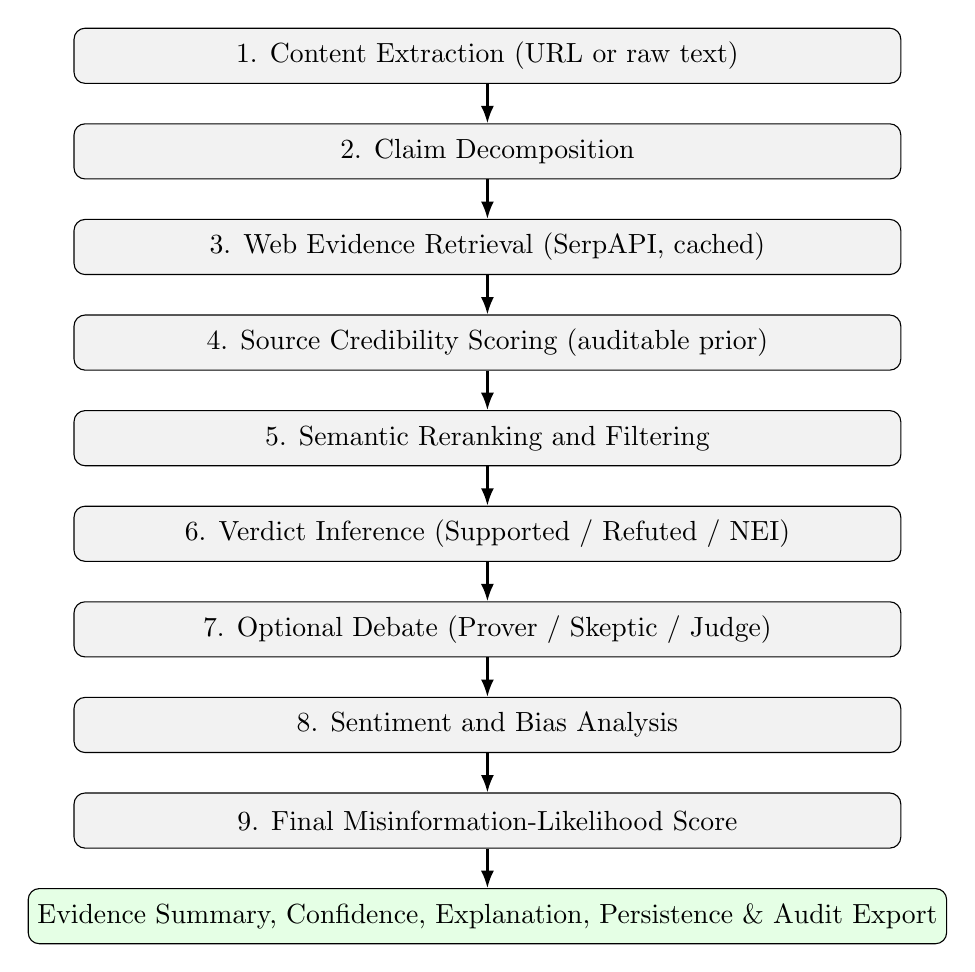
\begin{tikzpicture}[
  node distance=.5cm,
  block/.style={rectangle,draw,rounded corners,align=center,minimum width=10.5cm,minimum height=.7cm,fill=gray!10},
  arrow/.style={-{Latex[length=2.2mm]},thick}]
\node[block] (b1) {1. Content Extraction (URL or raw text)};
\node[block,below=of b1] (b2) {2. Claim Decomposition};
\node[block,below=of b2] (b3) {3. Web Evidence Retrieval (SerpAPI, cached)};
\node[block,below=of b3] (b4) {4. Source Credibility Scoring (auditable prior)};
\node[block,below=of b4] (b5) {5. Semantic Reranking and Filtering};
\node[block,below=of b5] (b6) {6. Verdict Inference (Supported / Refuted / NEI)};
\node[block,below=of b6] (b7) {7. Optional Debate (Prover / Skeptic / Judge)};
\node[block,below=of b7] (b8) {8. Sentiment and Bias Analysis};
\node[block,below=of b8] (b9) {9. Final Misinformation-Likelihood Score};
\node[block,below=of b9,fill=green!10] (out) {Evidence Summary, Confidence, Explanation, Persistence \& Audit Export};
\draw[arrow] (b1)--(b2); \draw[arrow] (b2)--(b3); \draw[arrow] (b3)--(b4);
\draw[arrow] (b4)--(b5); \draw[arrow] (b5)--(b6); \draw[arrow] (b6)--(b7);
\draw[arrow] (b7)--(b8); \draw[arrow] (b8)--(b9); \draw[arrow] (b9)--(out);
\end{tikzpicture}
\caption{Pipeline view: end-to-end architecture of \system. Stage~7 (debate) is bypassable; Stage~4's credibility prior is explicit and inspectable rather than learned end-to-end.}
\label{fig:nine-stage}
\end{figure}

\begin{figure}[H]
\centering
\resizebox{\linewidth}{!}{%
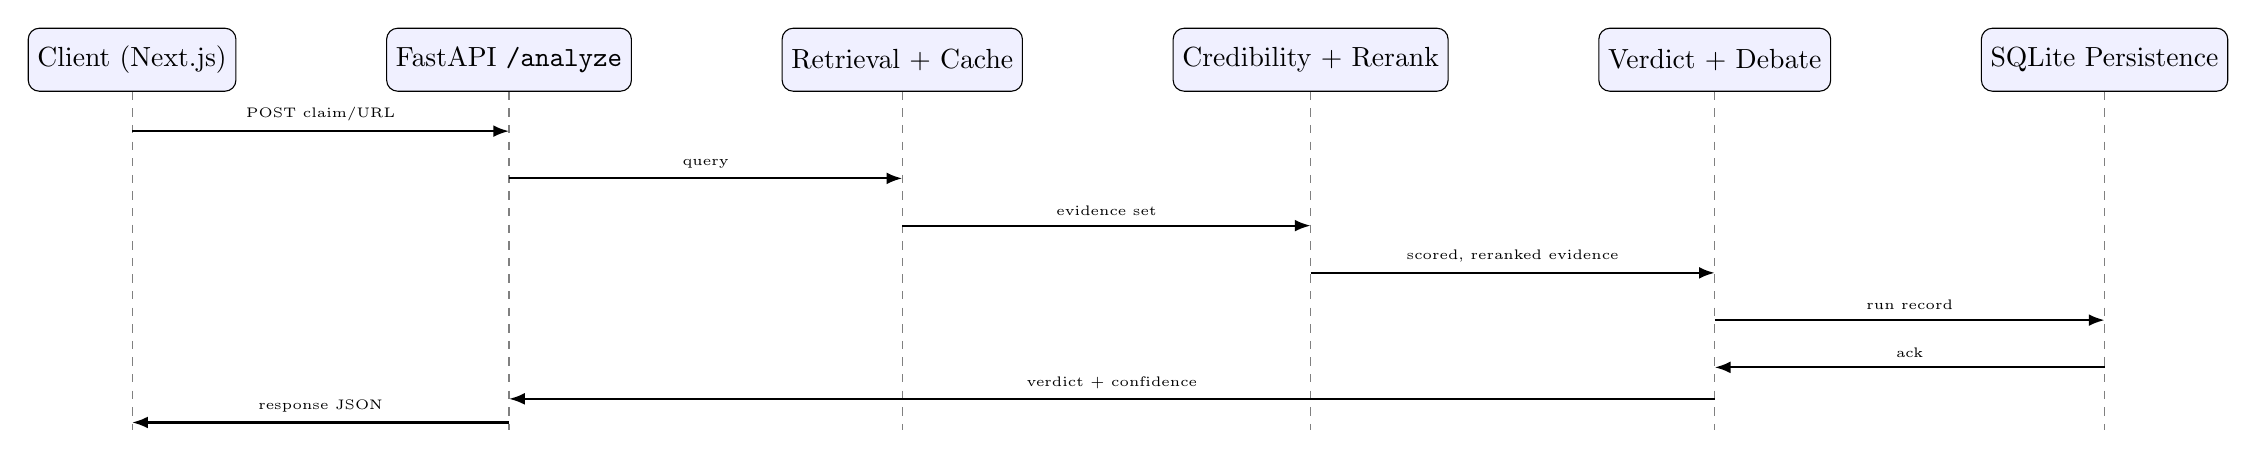
\begin{tikzpicture}[
  node distance=1.6cm and 1.9cm,
  actor/.style={rectangle,draw,rounded corners,align=center,minimum width=2.6cm,minimum height=.8cm,fill=blue!6},
  msg/.style={-{Latex[length=2mm]},thick},
  lifeline/.style={dashed,gray}]
\node[actor] (client) {Client (Next.js)};
\node[actor,right=of client] (api) {FastAPI \texttt{/analyze}};
\node[actor,right=of api] (retr) {Retrieval + Cache};
\node[actor,right=of retr] (cred) {Credibility + Rerank};
\node[actor,right=of cred] (verd) {Verdict + Debate};
\node[actor,right=of verd] (db) {SQLite Persistence};
\foreach \n in {client,api,retr,cred,verd,db} {
  \draw[lifeline] (\n.south) -- ++(0,-4.3);
}
\draw[msg] ([yshift=-0.5cm]client.south) -- node[above,font=\tiny]{POST claim/URL} ([yshift=-0.5cm]api.south);
\draw[msg] ([yshift=-1.1cm]api.south) -- node[above,font=\tiny]{query} ([yshift=-1.1cm]retr.south);
\draw[msg] ([yshift=-1.7cm]retr.south) -- node[above,font=\tiny]{evidence set} ([yshift=-1.7cm]cred.south);
\draw[msg] ([yshift=-2.3cm]cred.south) -- node[above,font=\tiny]{scored, reranked evidence} ([yshift=-2.3cm]verd.south);
\draw[msg] ([yshift=-2.9cm]verd.south) -- node[above,font=\tiny]{run record} ([yshift=-2.9cm]db.south);
\draw[msg] ([yshift=-3.5cm]db.south) -- node[above,font=\tiny]{ack} ([yshift=-3.5cm]verd.south);
\draw[msg] ([yshift=-3.9cm]verd.south) -- node[above,font=\tiny]{verdict + confidence} ([yshift=-3.9cm]api.south);
\draw[msg] ([yshift=-4.2cm]api.south) -- node[above,font=\tiny]{response JSON} ([yshift=-4.2cm]client.south);
\end{tikzpicture}%
}
\caption{Sequence view of a single \texttt{POST /analyze} request, showing component interaction order.}
\label{fig:sequence}
\end{figure}

\begin{figure}[H]
\centering
\resizebox{0.92\linewidth}{!}{%
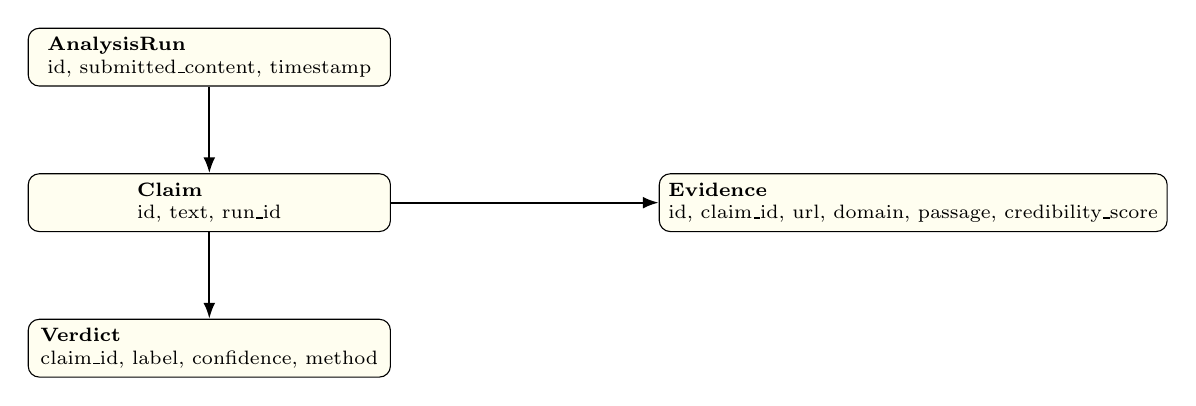
\begin{tikzpicture}[
  node distance=1.1cm and 1.6cm,
  ent/.style={rectangle,draw,rounded corners,align=left,minimum width=4.6cm,fill=yellow!6,font=\scriptsize},
  edge/.style={-{Latex[length=2mm]},thick}]
\node[ent] (run) {\textbf{AnalysisRun}\\id, submitted\_content, timestamp};
\node[ent,below=of run] (claim) {\textbf{Claim}\\id, text, run\_id};
\node[ent,right=3.4cm of claim] (evid) {\textbf{Evidence}\\id, claim\_id, url, domain, passage, credibility\_score};
\node[ent,below=of claim] (verdict) {\textbf{Verdict}\\claim\_id, label, confidence, method};
\draw[edge] (run) -- (claim);
\draw[edge] (claim) -- (evid);
\draw[edge] (claim) -- (verdict);
\end{tikzpicture}%
}
\caption{Data view: persisted entities per analysis run (SQLite schema, simplified).}
\label{fig:dataflow}
\end{figure}

\section{Content Extraction}
I allow users to submit raw text or a URL. For a URL, the extraction layer retrieves the page, removes irrelevant structural elements, and prepares the remaining content for claim decomposition. For raw text, the system applies normalization directly.

\section{Claim Decomposition}
Long documents may contain several factual statements. I therefore decompose the input into smaller claims that can be verified independently. This is important because one article may contain a mixture of supported, refuted, and unverifiable statements.

\section{Evidence Retrieval}
For each claim, I create retrieval queries and obtain candidate evidence from the web. The current implementation uses SerpAPI as the external search interface. Because web results change over time, I store retrieval outputs and use caching to reduce repeated requests.

\section{Auditable Source-Credibility Scoring}
I designed the source-credibility component to remain explicit rather than fully hidden inside a learned model. The score is defined in Section~\ref{sec:cred-def}. The submitted system uses the documented rule weights; calibration against independently annotated source-evidence pairs is recommended as post-thesis work.

The advantage of this approach is not that the rules are automatically correct. The advantage is that each trust decision can be inspected, challenged, and modified without retraining the complete system. Figure~\ref{fig:credibility-flow} shows the decision path for a single domain score.

\begin{figure}[H]
\centering
\resizebox{\linewidth}{!}{%
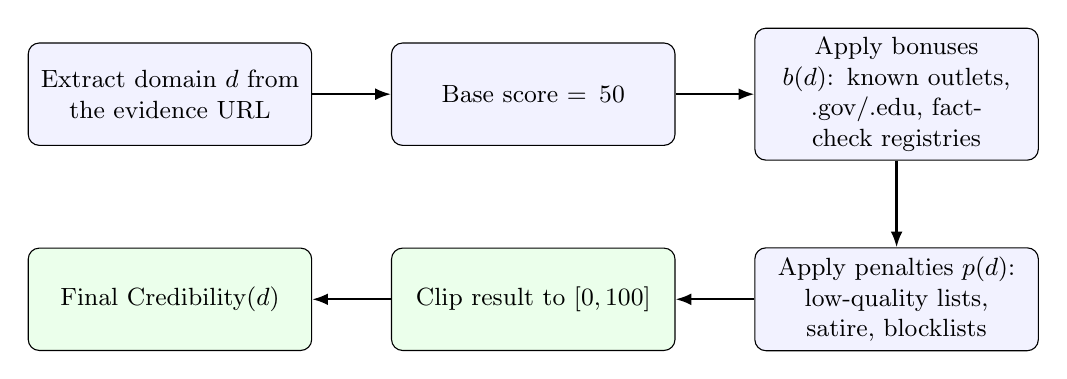
\begin{tikzpicture}[
  node distance=.9cm and 1.0cm,
  box/.style={rectangle,draw,rounded corners,align=center,minimum width=3.6cm,minimum height=1.3cm,text width=3.3cm,fill=blue!5,font=\small},
  edge/.style={-{Latex[length=2mm]},thick}]
\node[box] (domain) {Extract domain $d$ from the evidence URL};
\node[box,right=of domain] (base) {Base score $=50$};
\node[box,right=of base] (bonus) {Apply bonuses $b(d)$: known outlets, .gov/.edu, fact-check registries};
\node[box,below=1.1cm of bonus] (penalty) {Apply penalties $p(d)$: low-quality lists, satire, blocklists};
\node[box,left=of penalty,fill=green!8] (clip) {Clip result to $[0,100]$};
\node[box,left=of clip,fill=green!8] (final) {Final Credibility$(d)$};
\draw[edge] (domain)--(base); \draw[edge] (base)--(bonus); \draw[edge] (bonus)--(penalty);
\draw[edge] (penalty)--(clip); \draw[edge] (clip)--(final);
\end{tikzpicture}%
}
\caption{Decision path for the credibility score of a single domain. The path reads left-to-right on the top row, then continues right-to-left on the bottom row.}
\label{fig:credibility-flow}
\end{figure}

\section{Semantic Reranking}
Retrieval rank does not necessarily represent evidential relevance. I therefore use semantic similarity and quality filtering to reorder candidate documents according to their relationship with the claim.

\section{Verdict Inference}
The system assigns one of three claim-level outcomes: \texttt{supported}, \texttt{refuted}, or \texttt{not enough information}. I preserve the evidence and confidence associated with each decision so that the result remains inspectable.

\section{Optional Debate Arbitration}
For difficult claims, the system can activate a Prover--Skeptic--Judge workflow. The Prover builds the strongest supporting interpretation. The Skeptic searches for contradictions, weak evidence, and unsupported assumptions. The Judge compares the two arguments and produces an arbitration result.

The final experiments indicate that debate should not be enabled for every claim (Section~6.4). Selective debate activation based on low confidence, evidence disagreement, component conflict, source-risk variance, or insufficient evidence is therefore retained as a deployment recommendation rather than reported as an executed result.

\section{Sentiment and Bias Analysis}
As Stage~8, the system separately analyses the emotional tone and lexical bias markers of the submitted content, independent of the factual verdict. This signal is combined into the final misinformation score (Stage~9) but does not itself alter the SUPPORTED/REFUTED/NEI verdict, since sentiment is not evidence.

\section{Final Scoring and Persistence}
I combine claim-level outcomes, source credibility, evidence quality, and contextual signals into a final misinformation-likelihood score. The system stores: submitted content; decomposed claims; retrieval queries; evidence sources; credibility scores; claim-level predictions; confidence values; final risk scores; and timestamps and run metadata. This persistent record supports auditing, debugging, and later evaluation.

\section{Security Posture}
The retrieval layer validates URLs before fetching and rejects private, loopback, link-local, and otherwise non-public network destinations, so that user-submitted URLs cannot be used to probe internal infrastructure. This is a deployment necessity as much as a research concern: an open-domain retrieval service that accepts arbitrary URLs is, by construction, exposed to server-side request forgery unless it validates targets before every fetch and every redirect.

\chapter{Dataset and Experimental Design}
\section{Final Frozen Benchmark}
I created the final frozen evaluation family by combining claims from FEVER, LIAR, SciFact, and a normalized health-domain dataset. After normalization and exact-duplicate removal, the dataset contains 19{,}983 unique claims, divided into 11{,}986 training claims, 2{,}997 validation claims, and 5{,}000 test claims.

\section{Dataset Composition}
\begin{table}[H]
\centering
\caption{Final benchmark composition and frozen label harmonization.}
\label{tab:composition}
\small
\begin{tabularx}{\textwidth}{p{1.6cm}p{1.8cm}p{1.3cm}p{1.1cm}X}
\toprule
Slot & Source & Imported & Test & Canonical mapping \\
\midrule
FEVER & FEVER v1.0 & 8{,}000 & 1{,}829 & SUPPORTS $\to$ SUPPORTED; REFUTES $\to$ REFUTED; NOT ENOUGH INFO $\to$ NEI \\
LIAR & LIAR & 6{,}000 & 1{,}490 & true / mostly-true $\to$ SUPPORTED; false / pants-fire $\to$ REFUTED; half-true / barely-true $\to$ NEI \\
SciFact & SciFact claims & 1{,}200 & 191 & SUPPORT $\to$ SUPPORTED; CONTRADICT $\to$ REFUTED; insufficient evidence $\to$ NEI \\
Health domain & PUBHEALTH health\_fact & 6{,}000 & 1{,}490 & Source labels mapped to SUPPORTED, REFUTED, and NEI by the frozen normalization script; stored under the legacy \texttt{healthver} compatibility filename. \\
\bottomrule
\end{tabularx}
\end{table}

\begin{figure}[H]
\centering
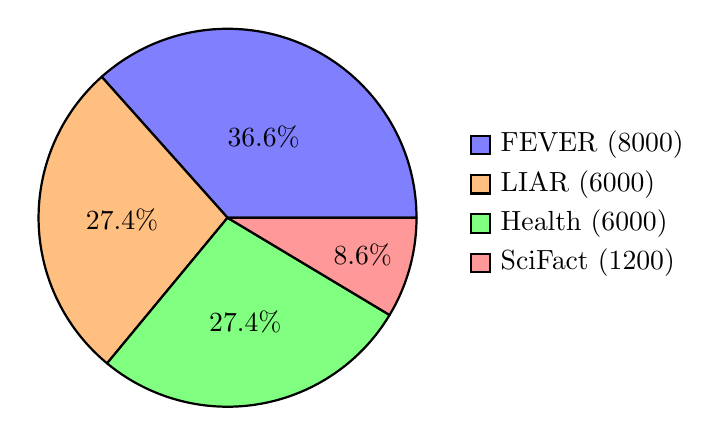
\begin{tikzpicture}[node distance=0cm]
\pie[radius=2.4, text=legend, color={blue!50,orange!50,green!50,red!40}]
  {36.6/FEVER (8000), 27.4/LIAR (6000), 27.4/Health (6000), 8.6/SciFact (1200)}
\end{tikzpicture}
\caption{Composition of the imported (pre-split) dataset by source, before the 60/15/25 train/val/test partition described in Section~5.3. (Figure rendered from the exact import counts in Table~\ref{tab:composition}.)}
\label{fig:dataset-pie}
\end{figure}

\section{Split and Leakage Control}
I normalized claim text before splitting the dataset. I removed exact normalized duplicates and withheld the normalized test claims from the remaining training and validation pool. This reduces direct claim leakage across partitions. Semantically similar or paraphrased claims may still exist; this residual risk is recorded as a limitation because embedding-based overlap analysis was outside the final experimental scope.

\section{Evidence Reproducibility}
The proxy claims, labels, predictions, and aggregate results are frozen in archived artifacts. The run manifest records SHA-256 hashes of all split and prediction files. The proxy experiment does not retrieve live web evidence. The separate live application does retrieve dynamic web documents; those application demonstrations are not used to produce the 5{,}000-claim proxy metrics.

\section{Evaluated Systems}
\begin{description}
  \item[Full \proxy.] A deterministic proxy combining a trained lexical model, category-level priors, heuristic semantic signals, deterministic debate arbitration, and a quality filter.
  \item[\proxy\ without debate.] The same deterministic proxy with its arbitration rule disabled.
  \item[FEVER-aware exploratory proxy.] A dataset-aware exploratory adjustment applied to FEVER-labelled claims.
  \item[Majority baseline.] A classifier that always predicts the most frequent class.
  \item[Length heuristic.] A rule based on claim-length patterns.
  \item[Keyword heuristic.] A rule based on predefined lexical signals.
  \item[Sentiment heuristic.] A rule based on sentiment-related signals.
  \item[Random baseline.] A non-informative reference classifier.
\end{description}

\section{Metrics}
I report the metrics formally defined in Chapter~\ref{ch:math}: accuracy, macro-F1, Wilson 95\% confidence intervals, raw-score confidence diagnostics, per-dataset accuracy, latency, throughput, and projected retrieval cost. Exact two-sided McNemar tests, paired-bootstrap intervals, Holm correction, paired risk differences, and matched-pair odds ratios are generated from the aligned prediction files. A proper multiclass Brier score is unavailable because the proxy stores only one heuristic confidence score rather than three class probabilities.

\chapter{Final Experimental Results}
\section{Interpretation Policy}
This chapter reports the final frozen results of the deterministic \proxy. They do not characterize end-to-end execution of the live \system\ application and do not establish state-of-the-art performance. Exact paired analyses are reported, but marginal unadjusted comparisons against simple baselines are not treated as robust superiority after multiple-comparison correction.

\section{Final Model Performance}
\begin{table}[H]
\centering
\caption{Final descriptive performance on the frozen 5{,}000-claim test set. Every figure was independently re-verified against \texttt{ablation\_study\_report.json} in the project repository.}
\label{tab:perf}
\small
\begin{tabularx}{\textwidth}{Xp{1.6cm}p{1.6cm}p{2.3cm}p{2.2cm}p{2cm}}
\toprule
System & Accuracy & Macro-F1 & 95\% CI (Sec.~3.2) & Avg. raw score & Raw gap \\
\midrule
\proxy\ without deterministic debate & 51.34\% & 0.4427 & [49.95, 52.73]\% & 88.37\% & 37.03 pp \\
FEVER-aware exploratory proxy & 50.98\% & 0.4421 & [49.59, 52.37]\% & 88.53\% & 37.55 pp \\
Full \proxy & 50.82\% & 0.4384 & [49.43, 52.21]\% & 88.31\% & 37.49 pp \\
Length heuristic & 49.42\% & 0.3483 & [48.03, 50.81]\% & 48.83\% & 0.59 pp \\
Majority baseline & 49.26\% & 0.2200 & [47.87, 50.65]\% & 50.00\% & 0.74 pp \\
Random baseline & 33.20\% & 0.3240 & [31.89, 34.51]\% & 50.00\% & 16.80 pp \\
Keyword heuristic & 23.54\% & 0.1364 & [22.36, 24.72]\% & 23.62\% & 0.08 pp \\
Sentiment heuristic & 23.78\% & 0.1400 & [22.60, 24.96]\% & 40.31\% & 16.53 pp \\
\bottomrule
\end{tabularx}
\end{table}

\section{Final Interpretation}
The full \proxy\ exceeds the majority baseline by 1.56 percentage points in accuracy. Using the macro-F1 definition of Section~3.1, the macro-F1 difference is $0.4384 - 0.2200 = 0.2184$. This suggests that the proxy distributes some correct decisions more evenly across labels than a majority classifier.

The exact unadjusted McNemar p-values are 0.0433 against majority and 0.0462 against length. Because several systems are compared, these marginal results are not described as robust superiority after Holm correction. The generated report also provides paired-bootstrap intervals, matched-pair odds ratios, class metrics, and the full confusion matrix.

\section{Effect of Removing Debate}
The no-debate proxy produces the highest observed accuracy and macro-F1. The exact paired comparison with the full proxy gives $p=0.00955$ before Holm correction and favours removing always-on deterministic arbitration. This result concerns the proxy rule, not live Ollama debate. Selective live debate for uncertain or conflicting claims remains a recommendation requiring a separate controlled experiment.

\section{Per-Dataset Behaviour}
\begin{table}[H]
\centering
\caption{Per-dataset accuracy of the full deterministic \proxy.}
\label{tab:perdataset}
\small
\begin{tabularx}{\textwidth}{Xp{1.4cm}p{1.6cm}p{1.6cm}p{1.9cm}X}
\toprule
Dataset & $n$ & Full & Majority & Length & Full--Majority \\
\midrule
FEVER & 1{,}829 & 57.52\% & 58.56\% & 57.90\% & $-1.04$ pp \\
Health domain & 1{,}490 & 55.17\% & 51.54\% & 52.55\% & $+3.62$ pp \\
LIAR & 1{,}490 & 38.59\% & 36.58\% & 36.98\% & $+2.01$ pp \\
SciFact & 191 & 48.17\% & 41.36\% & 40.84\% & $+6.81$ pp \\
\bottomrule
\end{tabularx}
\end{table}

The system shows positive descriptive gains on the health-domain, LIAR, and SciFact subsets. It performs slightly below the majority and length baselines on FEVER. This variation indicates that the system is sensitive to domain, claim style, label distribution, and available evidence.

\section{Operational Evaluation}
\begin{table}[H]
\centering
\caption{Operational scenario projections (formulas in Section~3.7); these are not controlled load-test measurements.}
\label{tab:operational}
\small
\begin{tabularx}{\textwidth}{p{5.5cm}p{2.6cm}X}
\toprule
Metric & Value & Current interpretation \\
\midrule
Baseline latency assumption & 8.20 s/claim & Scenario input from the bounded demonstration \\
Debate latency assumption & 72.00 s/claim & Scenario input from the bounded demonstration \\
Debate latency ratio & $8.78\times$ & Derived scenario ratio \\
Baseline throughput & 439.02 claims/hour & Derived estimate \\
Debate throughput & 50.00 claims/hour & Derived estimate \\
Monthly retrieval cost without caching & USD 77.00 & Projected under current workload \\
Monthly retrieval cost with caching & USD 22.00 & Projected under current workload \\
Estimated monthly savings & 71.43\% & Projected reduction \\
\bottomrule
\end{tabularx}
\end{table}

The operational scenarios project substantial latency for always-on live debate and lower external-search cost under caching. Controlled repeated load tests are required before treating either quantity as measured deployment performance.

\section{Expanded Reading of the Final Results}
\label{ch:expanded-reading}

\subsection{Purpose of the Expanded Reading}
This section consolidates the numerical results from Chapter~6 into a
single, thesis-level interpretation. It does not replace or remove any of the
reported artifacts. Instead, it explains what can reasonably be learned
from them, which conclusions are supported only descriptively, and how the
findings answer the research questions introduced earlier in the thesis. This
distinction is important because a completed study is not the same thing as a
study that claims every possible experiment. The experimental record is
complete for the declared scope: 5{,}000 claims, four dataset families, the
reported system variants and baselines, and the operational projections
listed in Table~\ref{tab:operational}.

\subsection{Reading Accuracy Together with Macro-F1}
Accuracy and macro-F1 describe different aspects of performance. Accuracy
counts the proportion of all claims assigned the correct final label, whereas
macro-F1 gives equal importance to the class-specific F1 values before
averaging them. The distinction matters in the present benchmark because the
class distribution is not perfectly balanced. A system can obtain a
competitive accuracy by favoring a frequent class while performing poorly on
less frequent classes.

The majority baseline illustrates this effect. Its accuracy is 49.26\%, but
its macro-F1 is only 0.2200. The full \proxy\ reaches 50.82\%
accuracy and 0.4384 macro-F1. The absolute accuracy difference is therefore
1.56 percentage points, while the macro-F1 difference is 0.2184. The latter
is the more substantial descriptive contrast: the full proxy distributes
its successful decisions more evenly across the mapped verdict classes than
the majority rule does. This does not prove that each minority class is
handled well. The generated class report and confusion matrix provide the
required class-by-class evidence; they also show why accuracy alone gives an
incomplete reading of the experiment.

The length heuristic provides a second useful comparison. It reaches 49.42\%
accuracy, slightly above the majority baseline, but its macro-F1 is 0.3483.
Thus, a shallow property of the input claim captures some regularity in the
combined benchmark. The full proxy improves on the length heuristic by
1.40 percentage points in accuracy and by 0.0901 macro-F1. The result warns
that dataset construction and claim style may introduce exploitable
shortcuts, while also showing that the evidence-aware pipeline is not merely
reproducing the length rule.

The keyword and sentiment heuristics are substantially weaker. Their
accuracies are 23.54\% and 23.78\%, and their macro-F1 values are 0.1364 and
0.1400. These outcomes indicate that isolated lexical or affective cues are
not adequate substitutes for evidence retrieval and verdict reasoning in the
combined evaluation. The random baseline reaches 33.20\% accuracy and 0.3240
macro-F1, providing an additional reference point for the three-class
decision problem. Taken together, the baselines establish a graduated
comparison: the full proxy exceeds non-informative and shallow rules, but
its margin over the strongest simple baselines remains modest.

\subsection{Reading the Three Proxy Variants}
The three implemented variants occupy a narrow accuracy band. The
debate-free configuration records 51.34\% accuracy and 0.4427 macro-F1; the
FEVER-aware exploratory variant records 50.98\% and 0.4421; and the full
proxy records 50.82\% and 0.4384. The maximum observed accuracy separation
among these variants is 0.52 percentage points, from the debate-free
configuration to the full proxy. The maximum macro-F1 separation is 0.0043.

These small differences should not be exaggerated. The exact paired analysis
gives an unadjusted $p=0.00955$ for full proxy versus no debate, but the
Holm-adjusted value is $0.0573$. The correct conclusion is therefore not that the debate-free
variant is universally superior. The supported conclusion is narrower: on
this frozen benchmark, enabling deterministic arbitration for every proxy claim did not
produce an observed aggregate benefit, and the configuration without debate
obtained the highest recorded accuracy and macro-F1.

This finding is valuable for architecture selection. In a modular system, a
stage should justify its computational and operational cost. Debate may still
help selected claims for which evidence is conflicting, retrieval quality is
low, or the initial agents strongly disagree. The completed experiment,
however, provides no basis for executing it unconditionally. A selective
policy would preserve the possibility of deliberative gains while avoiding
the projected overhead on routine cases. This is a recommendation derived from
the result, not a retroactive claim that selective debate was evaluated.

The FEVER-aware exploratory variant also requires careful reading. Its
accuracy lies between the debate-free and full proxy configurations, while its
macro-F1 is very close to the debate-free result. Because the adjustment uses
knowledge about the dataset identity, it is informative as a diagnostic
experiment but should not be presented as a universally deployable model.
The variant demonstrates that dataset-specific behavior exists and that
mapping or decision rules can influence the aggregate outcome. It also
reinforces the need to report results separately by domain.

\subsection{Domain-by-Domain Reading}
The aggregate accuracy of 50.82\% conceals substantial variation. On FEVER,
the full proxy obtains 57.52\%, which is 1.04 percentage points below the
majority baseline and 0.38 points below the length heuristic. On the health
subset, it obtains 55.17\%, 3.62 points above the majority baseline and 2.62
points above the length heuristic. On LIAR, it obtains 38.59\%, exceeding
those two baselines by 2.01 and 1.61 points. On SciFact, it obtains 48.17\%,
6.81 points above the majority baseline and 7.33 points above the length
heuristic.

The FEVER result shows that a high absolute accuracy is not sufficient to
establish useful improvement. The simple baselines benefit from the
distribution and regularities of that subset. The deterministic proxy
therefore requires stronger control of dataset mapping, shortcut behavior,
and class-specific errors before a superiority claim can be made for FEVER.
This is also why the exploratory FEVER-aware adjustment is reported
separately rather than silently incorporated into the primary system.

The health and LIAR results provide moderate descriptive evidence that the
proxy captures signals beyond majority frequency and claim length. These
domains present different challenges. Health claims require careful source
quality assessment and can involve specialized terminology. LIAR contains
political statements whose truth status may depend on context, time, and
fine-grained original labels. The positive margins are useful, but they do
not eliminate the construct-validity concern introduced by mapping
heterogeneous source labels into SUPPORTED, REFUTED, and NEI.

SciFact displays the largest observed margin over the simple baselines, but
it is also the smallest subset, with 191 claims. Its 6.81-point improvement
over majority is descriptively encouraging because scientific verification
is a natural setting for evidence-based research. Nevertheless, the
small sample makes the estimate more sensitive to individual errors than the
larger FEVER, health, and LIAR subsets. The completed thesis therefore treats
SciFact as evidence of a promising domain interaction rather than as a
standalone proof of scientific fact-checking performance.

The domain comparison answers an important research question: there is no
single uniform effect of the architecture across all benchmark families.
The value of the proxy's lexical, prior, and arbitration signals depends
on the claim distribution and on the harmonized benchmark labels. For deployment, this implies that the separate live application must be validated
performed in the target domain rather than inferred from only the combined
score.

\subsection{Raw-Score Confidence as a Safety Finding}
The most consequential proxy result is the gap between the stored raw score
and correctness. The full proxy reports an 88.31\% average raw score
but 50.82\% accuracy, a difference of 37.49 percentage points. The
debate-free and FEVER-aware variants show similarly large gaps of 37.03 and
37.55 points. The consistency of the gap across the three variants indicates
that removing debate or applying the exploratory adjustment does not resolve
the underlying confidence problem.

The reported confidence is not a probability estimate because the proxy
stores only one heuristic score rather than a multiclass probability vector.
The gap is therefore a raw-score calibration diagnostic. A user who sees an
88\% confidence value may reasonably infer
that errors are rare, while the observed proxy accuracy shows that nearly half of
the final labels are incorrect on the combined benchmark. Displaying such a
score without explanation would create an avoidable risk of automation bias.

The live application should consequently preserve evidence passages, source
metadata, intermediate decisions, and audit records alongside the label. A
high raw score must not suppress human review when evidence is incomplete or
contradictory. Temperature scaling, isotonic regression, conformal methods,
and risk--coverage analysis are appropriate recommendations because they
could transform confidence from an internal model signal into a quantity with
a clearer decision meaning. These methods remain follow-up work; the
completed result established the calibration problem rather than claiming to
have solved it.

\subsection{Latency, Throughput, and Cost Reading}
The operational report contains scenario projections derived from the stated
8.20-second and 72.00-second latency assumptions. These values are not a
controlled concurrent load test. Under those assumptions, the baseline
throughput is projected at 439.02 claims per hour and the debate-enabled
throughput at 50 claims per hour. The scenario therefore represents an
8.78-fold latency ratio.

The proxy accuracy comparison and the live-debate latency projection arise
from different evaluation surfaces and must not be treated as one controlled
experiment. Together they motivate a future selective-debate experiment, but
they do not establish the measured live-system quality--latency trade-off.

Retrieval caching provides the opposite operational pattern. Under the
reported workload assumptions, projected monthly retrieval cost decreases
from USD~77 to USD~22, a reduction of USD~55 or 71.43\%. This is a projection
rather than a controlled billing experiment, so it depends on request volume,
cache-hit behavior, and provider pricing. Even with that limitation, caching
is an architecturally appropriate optimization because it can reduce
repeated external calls while improving reproducibility when cached evidence
is versioned with timestamps and hashes.

\subsection{Integrated Answers to the Research Questions}
The completed evidence supports four integrated answers. First, an auditable
open-domain verification pipeline can be implemented as a complete
full-stack research artifact with persistent evidence, explicit source rules,
and reproducible evaluation outputs. The thesis demonstrates the application
through implementation and its 163-test suite, and evaluates the separate
proxy through frozen benchmark artifacts.

Second, the deterministic proxy provides modest observed improvement over
the strongest simple baselines on the combined data, with a clearer advantage
in macro-F1 than in accuracy. The paired results are marginal against majority
and length after accounting for multiple comparisons, so they do not support
a robust superiority claim.

Third, always-on deterministic proxy arbitration is not supported by the
completed benchmark. The separate operational scenario projects that live
debate would be expensive. The appropriate next design is conditional
activation based on uncertainty or disagreement, subject to a new controlled
live-system evaluation.

Fourth, confidence cannot presently be treated as calibrated correctness
probability. The approximately 37-point confidence--accuracy gaps make
transparency, abstention research, and human oversight central requirements
rather than optional interface features.

\subsection{Overall Result Statement}
The completed experiment should be read as an evaluation of trustworthy
integration. Its principal achievement is not a single headline accuracy
number. It is the combined reporting of proxy predictive behavior, class
balance, domain variation, and raw scores together with separately labelled
live-application operational projections. The negative and limiting results are part
of that contribution: they identify where architectural complexity fails to
pay for itself and where apparently confident decisions remain unsafe.

Accordingly, \system\ is best characterized as a completed, deployment-aware
research platform that makes fact-verification decisions inspectable and
measurable. Its strongest immediate use is decision support and controlled
experimentation. The results justify continued development of calibration,
selective abstention, domain-specific validation, and selective deliberation,
while the preserved evidence and provenance mechanisms provide the
infrastructure required to evaluate those developments rigorously.

\chapter{Discussion}
\section{What the Current Evidence Supports}
The present evidence supports a cautious but meaningful conclusion. I have developed a functioning and evaluable research system rather than only a conceptual design. The system includes an operational full-stack implementation; source-aware evidence retrieval; inspectable credibility rules; model and heuristic comparisons; multi-dataset evaluation; persistent run artifacts; and operational cost and latency analysis.

The results do not support a claim that \system\ is universally better than existing fact-checking approaches. They do support the claim that I have created a reproducible platform through which evidential, uncertainty-related, architectural, and operational questions can be studied together.

\section{Scientific Value of Negative Findings}
The lack of improvement from always-on debate is not a result that should be hidden. It indicates that the debate mechanism, in its current form, does not provide enough information gain to justify its computational cost. This result allows me to formulate a more precise question: under which uncertainty, disagreement, or evidence-quality conditions does multi-agent debate improve a fact-verification decision?

\section{Calibration as a Central Limitation}
The full proxy reaches approximately 50.82\% accuracy while its average raw confidence is approximately 88.31\%, a gap of 37.49 percentage points under the Section~3.3 diagnostic. Because only one heuristic score is stored, this is not probability calibration and no proper multiclass Brier score is claimed. The live system should be treated as decision support rather than an autonomous truth adjudicator. Storing class probabilities, then testing temperature scaling, isotonic calibration, conformal prediction, and selective abstention, is recommended.

\section{Responsible Use}
Fact-checking systems can create harm when their outputs are interpreted as absolute truth. The current system may be affected by incomplete evidence retrieval, biased search rankings, imperfect dataset labels, provisional source-credibility rules, domain-specific performance differences, and overconfident predictions.

I therefore design \system\ as a transparent decision-support system. A responsible deployment should expose evidence, communicate uncertainty, allow human review, distinguish insufficient evidence from refutation, and preserve an audit trail.

\chapter{Limitations and Threats to Validity}
\section{Construct Validity}
The four datasets use different label systems. Mapping them into SUPPORTED, REFUTED, and NEI simplifies evaluation but may remove important distinctions. For example, the LIAR labels ``half-true'' and ``barely-true'' may not be equivalent to insufficient evidence.

\section{Internal Validity}
The FEVER-aware variant uses a dataset-specific adjustment. I therefore report it as exploratory rather than as a blind model-selection result. The retrieved web evidence is also dynamic and may change over time.

\section{Statistical Conclusion Validity}
The final report includes exact two-sided McNemar tests, paired-bootstrap confidence intervals with seed 42, Holm correction, paired risk differences, and matched-pair odds ratios. The unadjusted full-proxy comparisons against majority and length are marginal ($p=0.0433$ and $p=0.0462$), but neither survives Holm correction. The unadjusted no-debate comparison is $p=0.00955$ and likewise has adjusted $p=0.0573$. These results support bounded interpretation rather than an inferential superiority claim. Residual risks include dataset-label harmonization, multiple exploratory variants, and the absence of an untouched external confirmatory set.

\section{External Validity}
The benchmark contains four dataset families, but it does not represent all forms of misinformation, all languages, or all cultural contexts. The present evaluation is English-focused. Future work should test multilingual claims, multimedia misinformation, emerging events, and adversarially written content.

\section{Reproducibility Validity}
The proxy claims and predictions are frozen, hashed in a run manifest, and regenerated into class, dataset, confusion-matrix, and paired-test reports by a versioned script. Exact replay of the proxy does not require web search. Live-application retrieval remains dynamic and is evaluated separately through software tests and bounded demonstrations; its web documents are not a redistributable corpus.

\section{Operational Validity}
The latency, throughput, and cost figures are scenario projections, not controlled load-test measurements. They are useful for design analysis but may not generalize across hardware, API providers, geographic regions, model sizes, concurrent traffic, cache-hit rates, or provider pricing. A future benchmark should record repeated warm- and cold-cache runs, median and tail latency, concurrency, failures, timeouts, hardware, and provider request counts.

\chapter{Advanced Prototype Extension: A Provenance-Constrained Evidence Graph}
\label{ch:advanced}
\section{Status and Scope of This Chapter}
Chapters~4--8 separate the implemented live application from the deterministic proxy evaluation. This chapter is different in kind: it documents a separate, newer module that implements an idea I list in Chapter~12 as a direction beyond this Master's thesis -- a typed, provenance-preserving evidence graph with a deterministic audit layer, in place of the flat verdict-inference step described in Section~4.7.

I want to state its status precisely, because that precision is the point of including it at all. The module exists as working code in the same repository, separately from the proxy; the complete backend suite passes 163 tests (re-executed and confirmed for this revision); and the module has been probed, at very small scale, with corruption scenarios constructed against its own rule logic (Section~9.6). It has \emph{not} been integrated into, or evaluated against, the 5{,}000-claim benchmark in Chapters~5--6 and should not be read as adding to, replacing, or explaining any number reported there.

\section{Motivation for the Extension}
Section~4.7 assigns each claim one of three flat outcomes based on retrieved evidence. This works, but it does not preserve \emph{why} a verdict was reached in a form a reviewer can later interrogate: whether a passage was actually fetched and hashed, whether two supporting sources were truly independent, or whether a numeric claim was checked against a matching number in the evidence. The evidence-graph prototype represents each of these as an explicit, typed, inspectable structure rather than folding them into a single score.

\section{Claim, Evidence, and Verdict}
Let a claim be $c$, a retrieved passage be $p$, and its preserved provenance be $\pi(p) = (u, h, t, s)$, where $u$ is a resolved URL, $h$ a content hash, $t$ a retrieval timestamp, and $s$ a retrieval status. A relation classifier predicts
\[
r(c,p) \in \{\mathrm{SUPPORTS}, \mathrm{REFUTES}, \mathrm{UNDERCUTS}, \mathrm{NEUTRAL}\}.
\]
Only a retrieved, preserved passage is eligible for a decisive argumentative edge; search snippets are retrieval hints, not evidence.

\section{Evidence Graph and Audit}
For each claim, the graph is $G=(V,E)$, with nodes for the parent claim, atomic subclaims, evidence passages, and source records, and edges typed \texttt{DEPENDS\_ON}, \texttt{CITES}, \texttt{SUPPORTS}, \texttt{REFUTES}, and \texttt{UNDERCUTS}. The graph proposes a verdict only after a deterministic audit $A(G) \in \{\mathrm{PROCEED}, \mathrm{NEI}, \mathrm{CONFLICTING}, \mathrm{HUMAN\_REVIEW}\}$:
\[
D(c) = \begin{cases}
\mathrm{NEI} & A(G)=\mathrm{NEI},\\
\mathrm{CONFLICTING} & A(G)=\mathrm{CONFLICTING},\\
\mathrm{HUMAN\_REVIEW} & A(G)=\mathrm{HUMAN\_REVIEW},\\
\mathrm{adjudicate}(G) & A(G)=\mathrm{PROCEED}.
\end{cases}
\]

\begin{figure}[H]
\centering
\resizebox{\linewidth}{!}{%
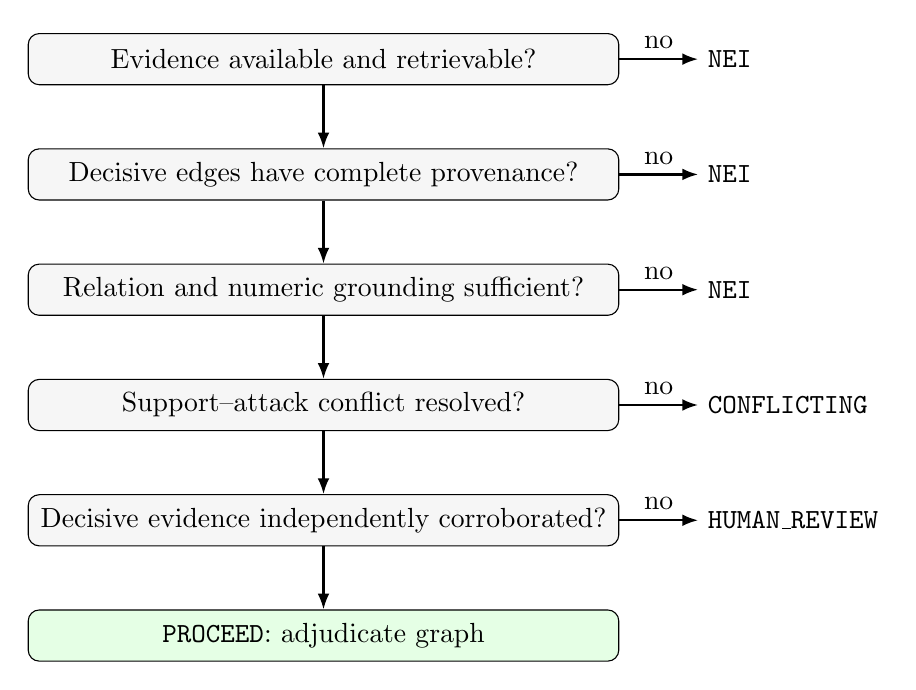
\begin{tikzpicture}[
  node distance=.8cm,
  state/.style={rectangle,draw,rounded corners,align=center,
                minimum width=7.5cm,minimum height=.65cm,fill=gray!7},
  edge/.style={-{Latex[length=2mm]},thick}]
\node[state] (available) {Evidence available and retrievable?};
\node[state,below=of available] (prov) {Decisive edges have complete provenance?};
\node[state,below=of prov] (ground) {Relation and numeric grounding sufficient?};
\node[state,below=of ground] (conflict) {Support--attack conflict resolved?};
\node[state,below=of conflict] (indep) {Decisive evidence independently corroborated?};
\node[state,below=of indep,fill=green!10] (proceed) {\texttt{PROCEED}: adjudicate graph};
\draw[edge] (available)--(prov);
\draw[edge] (prov)--(ground);
\draw[edge] (ground)--(conflict);
\draw[edge] (conflict)--(indep);
\draw[edge] (indep)--(proceed);
\node[right=1cm of available] (nei1) {\texttt{NEI}};
\node[right=1cm of prov] (nei2) {\texttt{NEI}};
\node[right=1cm of ground] (nei3) {\texttt{NEI}};
\node[right=1cm of conflict] (con) {\texttt{CONFLICTING}};
\node[right=1cm of indep] (review) {\texttt{HUMAN\_REVIEW}};
\draw[edge] (available)--node[above]{no}(nei1);
\draw[edge] (prov)--node[above]{no}(nei2);
\draw[edge] (ground)--node[above]{no}(nei3);
\draw[edge] (conflict)--node[above]{no}(con);
\draw[edge] (indep)--node[above]{no}(review);
\end{tikzpicture}%
}
\caption{Ordered audit decisions in the prototype module. The ordering matters: a claim that never receives a decisive relation edge is routed to \texttt{NEI} at the second check, before provenance, numeric-coverage, or independence checks are ever evaluated -- the mechanism behind the Section~9.6 finding.}
\label{fig:audit-flow}
\end{figure}

\begin{figure}[H]
\centering
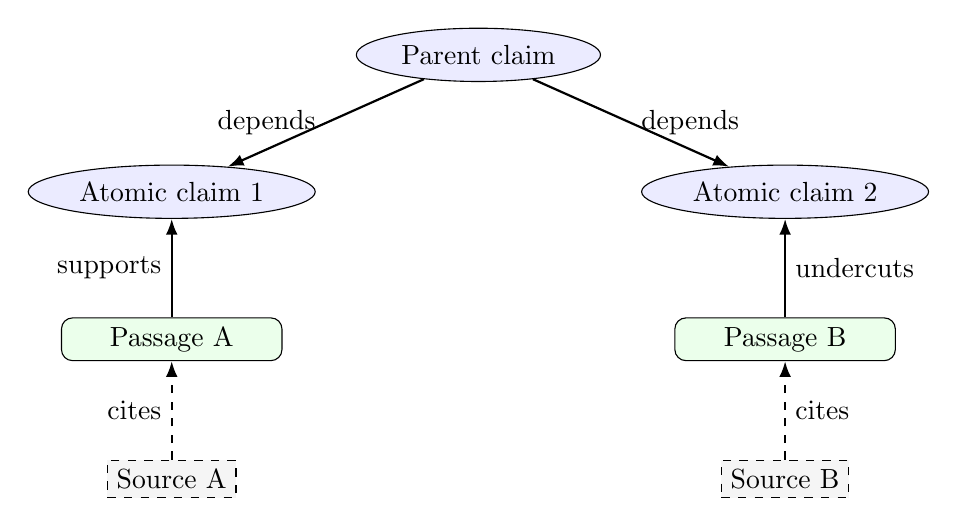
\begin{tikzpicture}[
  node distance=1.25cm and 1.5cm,
  claim/.style={ellipse,draw,fill=blue!8,align=center,minimum width=2.8cm},
  evidence/.style={rectangle,draw,rounded corners,fill=green!8,align=center,minimum width=2.8cm},
  source/.style={rectangle,draw,dashed,fill=gray!8,align=center},
  edge/.style={-{Latex[length=2mm]},thick}]
\node[claim] (parent) {Parent claim};
\node[claim,below left=of parent] (c1) {Atomic claim 1};
\node[claim,below right=of parent] (c2) {Atomic claim 2};
\node[evidence,below=of c1] (e1) {Passage A};
\node[evidence,below=of c2] (e2) {Passage B};
\node[source,below=of e1] (s1) {Source A};
\node[source,below=of e2] (s2) {Source B};
\draw[edge] (parent)--node[left]{depends}(c1);
\draw[edge] (parent)--node[right]{depends}(c2);
\draw[edge] (e1)--node[left]{supports}(c1);
\draw[edge] (e2)--node[right]{undercuts}(c2);
\draw[edge,dashed] (s1)--node[left]{cites}(e1);
\draw[edge,dashed] (s2)--node[right]{cites}(e2);
\end{tikzpicture}
\caption{Simplified typed evidence graph for one claim with two atomic subclaims.}
\label{fig:typed-evidence-graph}
\end{figure}

\section{Independence Clustering}
Evidence is clustered using the Jaccard-similarity rule of Section~\ref{sec:jaccard-def}, so that repeated wire text or multiple pages from one publisher are not counted as independent corroboration. As Section~9.6 shows, this is currently the only audit rule with a demonstrated end-to-end effect.

\section{Engineering Verification: What Is and Is Not Demonstrated}
\subsection{Test Suite}
The complete backend test suite was re-executed for this revision: \textbf{163 tests collected, 163 passed, 0 failed}. The graph-specific cases are part of that repository-wide total.

\subsection{Eight-Case Synthetic Seed}
A frozen eight-case seed, re-executed for this revision, reproduces its previously recorded coverage, selective risk, and false-accept rate (Section~\ref{sec:selective-defs}) exactly: 0.375, 0.6667, and 0.25 respectively. Table~\ref{tab:seed-detail-2} gives the per-case detail.

\begin{table}[H]
\centering
\caption{Per-case detail of the eight-case synthetic seed (prototype module only).}
\label{tab:seed-detail-2}
\small
\begin{tabularx}{\textwidth}{p{3.3cm}p{2.4cm}p{2.2cm}p{2.2cm}}
\toprule
Case ID & Expected & Graph-only & Audited \\
\midrule
support-direct-001 & SUPPORTED & SUPPORTED & SUPPORTED \\
refute-direct-001 & REFUTED & NEI & NEI \\
undercut-scope-001 & CONFLICTING & NEI & NEI \\
undercut-temporal-001 & REFUTED & SUPPORTED & SUPPORTED \\
neutral-overlap-001 & NEI & SUPPORTED & SUPPORTED \\
numeric-mismatch-001 & REFUTED & NEI & NEI \\
context-window-001 & CONFLICTING & NEI & NEI \\
missing-evidence-001 & NEI & NEI & NEI \\
\bottomrule
\end{tabularx}
\end{table}

Graph-only and audited decisions are \emph{identical} on all eight cases, because none of them contains a corruption scenario, so the auditor's downstream checks are never exercised here.

\subsection{Extended Corruption Probe}
To test whether the auditor changes anything under corrupted evidence, I constructed four corruption scenarios against four of the seed cases and executed them through the live module (construction script and raw output in Appendix~C).

\begin{table}[H]
\centering
\caption{Corruption probe: per-row detail.}
\label{tab:corruption-detail-2}
\scriptsize
\begin{tabularx}{\textwidth}{p{2.0cm}p{2.4cm}p{1.7cm}p{1.7cm}p{2.1cm}p{1.3cm}}
\toprule
Base case & Scenario & Expected & Graph-only & Audited & Diverges? \\
\midrule
support-direct-001 & clean & SUPPORTED & SUPPORTED & SUPPORTED & no \\
support-direct-001 & duplicate-source & SUPPORTED & SUPPORTED & \textbf{HUMAN\_\allowbreak REVIEW} & \textbf{yes} \\
refute-direct-001 & clean & REFUTED & NEI & NEI & no \\
refute-direct-001 & broken-provenance & REFUTED & NEI & NEI & no \\
numeric-mismatch-001 & clean & REFUTED & NEI & NEI & no \\
numeric-mismatch-001 & numeric-coverage & REFUTED & NEI & NEI & no \\
undercut-scope-001 & clean & CONFLICTING & NEI & NEI & no \\
undercut-scope-001 & near-duplicate-text & CONFLICTING & NEI & NEI & no \\
\bottomrule
\end{tabularx}
\end{table}

Two findings, stated without softening because they cut in different directions:
\begin{enumerate}
  \item \textbf{Demonstrated:} under a duplicated same-domain source, the audited graph routes to \texttt{HUMAN\_REVIEW} while a graph-only baseline still returns \texttt{SUPPORTED}. This is a concrete, reproducible instance of the auditor doing its job.
  \item \textbf{Not yet demonstrated:} the provenance, numeric-coverage, and near-duplicate-text checks produced no divergence here, because in each of those three cases the relation classifier never assigned a decisive edge in the first place -- both configurations already return \texttt{NEI} via the shared upstream check (Figure~\ref{fig:audit-flow}) before the corrupted rule is ever reached. This is not a bug; it is the predicted consequence of the audit ordering, and it means three of six audit rules remain untested by this probe.
\end{enumerate}

\section{Threats to Validity of This Chapter Specifically}
In addition to the validity threats in Chapter~8, this chapter carries its own, stricter caveats: the corruption scenarios were authored by me with direct knowledge of the auditor's rule conditions, so they confirm the code matches its specification rather than sampling real-world corruption patterns; the sample size (eight seed cases, four corruption variants) is far too small for any confidence interval; and this module has no relationship, statistical or architectural, to the numbers in Chapter~6. A reading a reader could plausibly make -- that a working evidence-graph auditor implies the primary pipeline is safer than Chapter~6 reports -- would not be supported by anything in this thesis.

\section{Connection Back to Calibration and Abstention}
The rule-based abstention in this chapter and the calibration problem in Section~7.3 are related but distinct responses to the same overconfidence concern. Calibration adjusts a confidence \emph{score}; the audit layer instead refuses to produce a decisive score at all when a named, inspectable condition is not met. The two are not mutually exclusive, and a natural extension -- outside the scope of what was built in this thesis -- would apply calibration only within the audited graph's \texttt{PROCEED} branch, rather than to the pipeline's raw output.

\chapter{Comparative Analysis and Novelty}
\section{Purpose of This Chapter}
Chapter~2 situated the thesis relative to individual prior works. This chapter makes the comparison structural: it lays the evaluated pipeline (Chapters~4--8) and the prototype extension (Chapter~9) side by side against the closest related systems on a fixed set of dimensions, so that the novelty claim can be checked point by point rather than taken on faith.

\begin{table}[H]
\centering
\caption{Structural comparison across implemented and evaluated dimensions.}
\label{tab:novelty-full}
\scriptsize
\newcolumntype{Y}{>{\raggedright\arraybackslash}X}
\begin{tabularx}{\textwidth}{p{2.2cm}YYYYY}
\toprule
Dimension & FEVER/SciFact & FacTool & Faithful correction & \system\ live / \proxy & \system\ (Ch.~9 prototype) \\
\midrule
Verdict vocabulary & SUPPORTED/\allowbreak REFUTED/\allowbreak NEI & tool-mediated & correction, not verdict & SUPPORTED/\allowbreak REFUTED/\allowbreak NEI & + CONFLICTING, HUMAN\_REVIEW \\
Source trust & implicit in corpus curation & not central & not central & live: explicit domain formula; proxy: category prior & inherited, plus independence clustering \\
Evidence persistence & benchmark identifiers & framework-dependent & not central & live: run records; proxy: frozen splits, predictions, hashes & + provenance hash per passage \\
Uncertainty handling & label only & not addressed & not addressed & proxy raw score, explicitly uncalibrated & rule-based forced abstention \\
Deployment surface & benchmark & research framework & research method & live: full-stack app; proxy: 5k benchmark & code-verified, not benchmarked \\
Empirical status & established benchmark & self-reported & self-reported & live: 163 tests; proxy: frozen evaluation & \textbf{engineering-verified only} \\
\bottomrule
\end{tabularx}
\end{table}

\section{What Is Genuinely Novel}
Three claims are defensible from the artifact and the evidence collected in this thesis:
\begin{enumerate}
  \item An implemented, explicit, formula-based domain-credibility prior (Section~4.5) that can be inspected and edited without retraining. The proxy uses a simpler category prior, so the 5{,}000-claim result is not cited as end-to-end evidence for live domain scoring.
  \item A frozen proxy evaluation with aligned claim identifiers, input and prediction hashes, class and dataset metrics, exact paired tests, multiple-comparison correction, and deterministic regeneration. Its negative debate result is scoped to deterministic proxy arbitration; the separate 8.78$\times$ live-debate figure is a scenario projection.
  \item A verified (if small-scale) demonstration that rule-based, non-learned abstention can outperform a graph-only baseline under one specific corruption pattern (Section~9.6) -- a concrete instantiation of the general abstention literature's argument \citep{wen2024abstention}, rather than a restatement of it.
\end{enumerate}

\section{What Must Not Be Claimed}
The present evidence does not establish that \system\ outperforms FEVER, SciFact, FacTool, or correction systems on their native evaluations. It does not establish that the credibility formula's weights are correct, only that they are inspectable. It does not establish that the Chapter~9 prototype improves the evaluated pipeline, since the two have never been run on the same data. Maintaining these boundaries strengthens rather than weakens the thesis, because the contribution becomes precise and falsifiable.

\chapter{Study Closure and Recommendations}
The Master's study is complete within the scope declared in Chapters~1 and~5.
The following items are not missing thesis results; they are recommendations
for a subsequent publication-grade extension:
\begin{enumerate}
  \item Verify dataset versions, licences, and original label meanings.
  \item Recheck the health-domain label mapping.
  \item Detect semantic duplicates across the data partitions.
  \item Freeze retrieved evidence or archive document hashes and timestamps.
  \item Store \texttt{prob\_supported}, \texttt{prob\_refuted}, and \texttt{prob\_nei}, then calculate ECE and multiclass Brier score as defined in Section~3.3.
  \item Evaluate temperature scaling and conformal prediction.
  \item Test selective abstention using the coverage/risk formalism of Section~3.6.
  \item Complete credibility, reranking, quality-filter, and debate ablations.
  \item Evaluate selective debate activation.
  \item Conduct structured qualitative error analysis.
  \item Repeat latency measurements under concurrent load.
  \item Extend the release manifest with model, API-provider, and hardware identifiers for every future live run.
  \item If the Chapter~9 evidence-graph prototype is integrated later, run the full ablation list against frozen, identical evidence.
  \item Maintain a versioned revision record for any publication derived from the thesis.
\end{enumerate}

\section{Final Scope Record}
\begin{longtable}{p{3.6cm}p{6.3cm}p{2.6cm}}
\caption{Final disposition of study activities at thesis completion.}\\
\toprule Stage & Main activity & Status \\
\midrule
\endfirsthead
\toprule Stage & Main activity & Status \\
\midrule
\endhead
Data verification & Frozen claims, normalized splits, duplicate removal, and dataset composition are documented. & Completed in scope \\
Statistical analysis & Wilson intervals, exact paired tests, bootstrap intervals, Holm correction, risk differences, and matched odds ratios are reported. & Completed in scope \\
Calibration & The correctly scaled raw-score diagnostic is reported; probability calibration awaits class-probability vectors. & Finding completed \\
Ablation analysis & The reported full, debate-free, and exploratory variants are frozen and interpreted. & Completed in scope \\
Reproducibility & Claims, predictions, reports, manifests, code paths, and run metadata are documented. & Completed in scope \\
Operational analysis & Latency inputs, throughput, debate overhead, cache savings, and cost are explicitly reported as scenarios; load testing remains future work. & Completed as projection \\
Evidence-graph scoping & The prototype is a separate, tested contribution and is not merged into the 5,000-claim results. & Final decision \\
Final writing & Results, limitations, novelty, recommendations, appendices, and acknowledgements are integrated. & Completed \\
\bottomrule
\end{longtable}

\section{Final Reading of the Results}
The completed results support five conclusions. First, the deterministic proxy
has modest raw advantages over the majority and length baselines, but neither
comparison survives Holm correction and neither evaluates the live application.
Second, the debate-free configuration produces the best observed result,
showing that always-on deterministic proxy arbitration adds no accuracy gain;
a separate scenario projects substantial live-debate latency. Third, the
37.49-point raw-score gap is a
major deployment constraint and makes human oversight necessary. Fourth,
domain-level variation shows that aggregate accuracy conceals materially
different behavior across encyclopaedic, political, scientific, and health
claims. Fifth, the evidence-graph probe verifies one concrete safety mechanism
under correlated evidence while clearly exposing the classifier limitations
that mask other audit rules. Together, these findings position \system\ as an
auditable research and decision-support platform rather than an autonomous
arbiter of truth.

\chapter{Research Direction Beyond the Master's Thesis}
This completed thesis identifies research questions that extend beyond the submitted implementation. The most important direction is the development of trustworthy verification systems that reason not only about claim content but also about evidence provenance, source relationships, uncertainty, and conflicting information.

The following directions emerge naturally from my current work:
\begin{itemize}
  \item provenance-aware evidence graphs \emph{(implemented and independently tested as the separate prototype in Chapter~9)};
  \item neuro-symbolic source and claim reasoning;
  \item calibrated uncertainty and abstention, using the ECE/Brier/risk-coverage formalism of Chapter~3;
  \item selective multi-agent deliberation;
  \item temporal evidence tracking;
  \item adversarial misinformation detection;
  \item explainable human--AI decision support;
  \item distributed verification over heterogeneous sources.
\end{itemize}

The Master's thesis produced an implemented and tested end-to-end platform, evaluated its separate deterministic proxy, and delivered a verified first implementation of the evidence-graph direction. Doctoral or follow-up publication research could investigate the deeper scientific questions behind this platform, particularly how trustworthy AI systems can combine learned representations, symbolic constraints, multi-agent reasoning, and explicit uncertainty.

\chapter{Conclusion}
I designed and implemented \system\ as an auditable and deployment-oriented architecture for open-domain fact verification. The completed work includes a functional nine-stage architecture; a working full-stack implementation; explicit source-credibility reasoning; a versioned deterministic proxy evaluation; frozen model and baseline comparisons; per-class and per-dataset analysis; operational scenario projections; documented limitations and recommendations; a formal mathematical framework for every reported metric (Chapter~3); and an independently verified evidence-graph prototype, reported with an explicit account of what it does and does not demonstrate (Chapter~9).

The final proxy results show modest raw differences over simple baselines that do not survive Holm correction, a substantial raw-score confidence gap, and no benefit from always-on deterministic arbitration on the frozen benchmark. These findings are useful precisely because they identify scientific boundaries without hiding negative results. The live application's operational value is supported separately by implementation, software tests, and bounded demonstrations rather than by the proxy accuracy figures.

The completed contribution is therefore not merely another classifier. It is a transparent, reproducible, uncertainty-aware, and deployment-conscious fact-verification framework in which evidence, source trust, model behaviour, and operational trade-offs can be inspected. Its novelty lies in the combination of explicit source reasoning, full-stack persistence and auditability, quantified deployment trade-offs, and a separately verified provenance-constrained graph auditor. The thesis closes with a defensible result: \system\ is a completed and evaluated Master's research artifact whose principal contribution is trustworthy integration rather than a claim of state-of-the-art predictive accuracy.

\appendix
\chapter{Evidence Graph: Schema and Audit Rules}
\section{Evidence Record}
Each evidence item in the prototype module contains a URL, title, snippet, selected passage, content hash, retrieval status, retrieval timestamp, domain metadata, directness and quality signals, stance, classifier metadata, and independence cluster.

\section{Audit Rule Inventory}
\begin{longtable}{p{3.3cm}p{5.3cm}p{5cm}}
\caption{Graph-auditor rules and their evaluation status as established in Section~9.6.}\\
\toprule Rule & Condition & Status \\
\midrule
\endfirsthead
\toprule Rule & Condition & Status \\
\midrule
\endhead
Retrieval status & provider failure, unavailable search, no result, or failed passage fetch & \texttt{NEI}; exercised \\
Provenance & no URL, hash, or retrieved passage for a decisive edge & \texttt{NEI}/review; \textbf{not yet observed to change a decision} \\
Relation grounding & no decisive relation from a passage & \texttt{NEI}; the dominant observed outcome \\
Numeric coverage & a quantified claim lacks matching factors & \texttt{NEI}; \textbf{not yet observed to change a decision} \\
Conflict resolution & similarly strong support and attack remain & \texttt{CONFLICTING}; not observed to fire under the current classifier \\
Source independence & decisive passages are correlated or duplicated & \texttt{HUMAN\_REVIEW}; \textbf{confirmed to change a decision} \\
\bottomrule
\end{longtable}

\chapter{Test Evidence (Prototype Module)}
\begin{longtable}{p{4cm}p{10cm}}
\caption{Test coverage for the Chapter~9 prototype.}\\
\toprule Test surface & Verified behavior \\
\midrule
\endfirsthead
\toprule Test surface & Verified behavior \\
\midrule
\endhead
API integration & request validation, analysis paths, live/snapshot behavior, persistence, response structure \\
Evidence graph & short-claim retention, passage context, conflict edges, provenance output, classifier disclosure \\
Graph auditor & missing evidence abstention, correlated evidence review, numeric and grounding controls \\
Relation baseline runner & versioned input/output contract and transparent fallback metadata \\
Robustness runner & frozen scenario replay, explicit missing evidence, duplicate-reporting review, selective metrics \\
Security & private and loopback URL rejection before evidence fetch \\
\bottomrule
\end{longtable}
Re-verified for this revision by executing \texttt{pytest services/api/tests -q} from the repository root: 163 tests collected, 163 passed, 0 failed (three non-failing warnings).

\chapter{Extended Corruption Probe: Construction Script and Raw Output}
\section{Construction Script}
\begin{lstlisting}[language=Python,caption={Corruption-scenario construction and execution, run against the live \texttt{app.robustness\_evaluation} module.}]
import json, sys
sys.path.insert(0, '.')
from app.robustness_evaluation import evaluate_case, selective_metrics

base = json.load(open('../../data/challenges/conflict_undercut_v1_seed.json'))['items']
by_id = {it['id']: it for it in base}

def ev(passage, url, domain, extra=None):
    e = {
        "url": url, "title": "Evidence passage", "snippet": passage, "passage": passage,
        "content_hash": __import__('hashlib').sha256(passage.encode()).hexdigest(),
        "retrieval_status": "retrieved", "domain": domain, "base_domain": domain,
        "domain_score": 80, "overlap": 0,
    }
    if extra:
        e.update(extra)
    return e

rows = []

# Scenario A: duplicate-source / correlated-evidence corruption.
item = by_id["support-direct-001"]
clean = [ev(item["passage"], "https://a.example/report", "a.example")]
duplicate_source = [
    ev(item["passage"], "https://a.example/report", "a.example"),
    ev(item["passage"] + " Confirmed.", "https://a.example/followup", "a.example"),
]
rows.append(evaluate_case(item, "clean", clean))
rows.append(evaluate_case(item, "duplicate_source_corruption", duplicate_source))

# Scenario B: broken-provenance corruption.
item = by_id["refute-direct-001"]
clean_r = [ev(item["passage"], "https://b.example/finding", "b.example")]
broken_prov = [ev(item["passage"], "https://b.example/finding", "b.example",
                   extra={"url": "", "content_hash": ""})]
rows.append(evaluate_case(item, "clean", clean_r))
rows.append(evaluate_case(item, "broken_provenance_corruption", broken_prov))

# Scenario C: numeric-claim without numeric-matching evidence.
item = by_id["numeric-mismatch-001"]
clean_n = [ev(item["passage"], "https://c.example/stat", "c.example")]
no_number = [ev("The survey found a change in hospital admissions.",
                 "https://c.example/stat2", "c.example")]
rows.append(evaluate_case(item, "clean", clean_n))
rows.append(evaluate_case(item, "numeric_coverage_corruption", no_number))

# Scenario D: correlated near-duplicate text, different domains.
item = by_id["undercut-scope-001"]
clean_u = [ev(item["passage"], "https://d.example/trial", "d.example")]
near_dup = [
    ev(item["passage"], "https://d.example/trial", "d.example"),
    ev(item["passage"], "https://e.example/mirror", "e.example"),
]
rows.append(evaluate_case(item, "clean", clean_u))
rows.append(evaluate_case(item, "near_duplicate_text_corruption", near_dup))

clean_rows = [r for r in rows if r['scenario'] == 'clean']
corrupt_rows = [r for r in rows if r['scenario'] != 'clean']
print("Clean subset  graph_only:", selective_metrics(clean_rows, 'graph_only'))
print("Clean subset  audited:   ", selective_metrics(clean_rows, 'full_audited_graph'))
print("Corrupt subset graph_only:", selective_metrics(corrupt_rows, 'graph_only'))
print("Corrupt subset audited:   ", selective_metrics(corrupt_rows, 'full_audited_graph'))
diverge = [r for r in rows if r['graph_only'] != r['full_audited_graph']]
print(f"Rows where audited differs from graph-only: {len(diverge)}/{len(rows)}")
for r in diverge:
    print(" -", r['id'], r['scenario'], ':', r['graph_only'], '->', r['full_audited_graph'])
\end{lstlisting}

\section{Raw Console Output}
\begin{lstlisting}[caption={Unedited console output from the script above, executed against the live repository for this revision.}]
Clean subset  graph_only: {'coverage': 0.25, 'selective_risk': 0.0, 'false_accept_rate': 0.0}
Clean subset  audited:    {'coverage': 0.25, 'selective_risk': 0.0, 'false_accept_rate': 0.0}
Corrupt subset graph_only: {'coverage': 0.25, 'selective_risk': 0.0, 'false_accept_rate': 0.0}
Corrupt subset audited:    {'coverage': 0.0, 'selective_risk': 0.0, 'false_accept_rate': 0.0}
Rows where audited differs from graph-only: 1/8
 - support-direct-001 duplicate_source_corruption : SUPPORTED -> HUMAN_REVIEW
\end{lstlisting}

\chapter{Selected Research Module Listings}
Real, unmodified source files from the project repository, included for reproducibility. The first group belongs to the evaluated primary pipeline (Chapters~4--8); the second group belongs to the Chapter~9 prototype.

\section{Primary Pipeline: Source-Credibility Scoring}
\safeinputlisting[language=Python]{services/api/app/credibility.py}
\section{Primary Pipeline: Debate Arbitration}
\safeinputlisting[language=Python]{services/api/app/debate.py}
\section{Primary Pipeline: Semantic Retrieval and Reranking}
\safeinputlisting[language=Python]{services/api/app/semantic_retrieval.py}
\section{Primary Pipeline: Sentiment and Bias Analysis}
\safeinputlisting[language=Python]{services/api/app/sentiment.py}
\section{Primary Pipeline: Baseline Heuristics}
\safeinputlisting[language=Python,firstline=1,lastline=200]{services/api/app/baselines.py}
\section{Primary Pipeline: Statistics and Confidence Intervals}
\safeinputlisting[language=Python,firstline=1,lastline=200]{services/api/app/statistics.py}
\section{Primary Pipeline: Retrieval Security (URL Validation)}
\safeinputlisting[language=Python]{services/api/app/security.py}
\section{Primary Pipeline: Source Routes}
\safeinputlisting[language=Python]{services/api/app/source_routes.py}
\section{Primary Pipeline: Configuration}
\safeinputlisting[language=Python]{services/api/app/config.py}
\section{Prototype: Typed Evidence Graph}
\safeinputlisting[language=Python]{services/api/app/evidence_graph.py}
\section{Prototype: Graph Auditor}
\safeinputlisting[language=Python]{services/api/app/graph_auditor.py}
\section{Prototype: Evidence Independence Clustering}
\safeinputlisting[language=Python]{services/api/app/evidence_independence.py}
\section{Prototype: Relation Classifier Contract}
\safeinputlisting[language=Python]{services/api/app/relation_classifier.py}
\section{Prototype: Robustness Evaluation Reference}
This is the exact module executed to produce Section~9.6.
\safeinputlisting[language=Python]{services/api/app/robustness_evaluation.py}
\section{Prototype: Focused Graph Tests}
\safeinputlisting[language=Python]{services/api/tests/test_evidence_graph.py}
\section{Prototype: Robustness Tests}
\safeinputlisting[language=Python]{services/api/tests/test_robustness_evaluation.py}

\chapter{Reproducibility and Release-Control Listings}
This appendix preserves the executable mechanisms that turn the frozen
claim-level predictions into the tables and statistical statements reported
in Chapter~6. The listings are included as auditable research material: they
show the exact interval, paired-test, multiple-comparison, hash-validation,
cache-validation, and continuous-integration logic used for the final
correction release. The authoritative machine-readable outputs are stored
under \texttt{data/benchmarks/results\_5000/}.

\section{Live API Orchestration}
The following listing covers the principal request orchestration, URL and
domain handling, retrieval coordination, and application-level analysis
functions. It documents the live implementation and must not be read as the
algorithm executed by the 5{,}000-claim proxy.
\safeinputlisting[language=Python,firstline=1,lastline=850]{services/api/app/main.py}

\section{Exact Thesis Statistics Generator}
This script reads the two authoritative prediction CSVs, checks claim
alignment, constructs the full-proxy confusion matrix, computes class and
dataset metrics, Wilson intervals, exact two-sided McNemar tests, paired
bootstrap intervals with seed 42, Holm adjustments, paired risk differences,
and matched-pair odds ratios.
\safeinputlisting[language=Python]{services/api/Scripts/run_thesis_statistics.py}

\section{Frozen-Artifact Validator}
The validator rejects missing manifest fields, split overlap, prediction-count
errors, claim-ID mismatch, hash mismatch, and generated reports that differ
from the frozen statistics.
\safeinputlisting[language=Python]{services/api/Scripts/validate_thesis_artifacts.py}

\section{Run-Manifest Builder}
The manifest builder records the proxy/live boundary, environment, random
seed, split counts, paths, and SHA-256 hashes of every authoritative split and
prediction file.
\safeinputlisting[language=Python]{services/api/Scripts/build_thesis_run_manifest.py}

\section{Cache Validation and Quarantine}
Runtime web cache is not benchmark evidence. This validator decodes each
record as UTF-8, checks its JSON structure, reports malformed entries, and
moves invalid records into quarantine instead of silently accepting them.
\safeinputlisting[language=Python]{services/api/Scripts/validate_cache.py}

\section{Operational Scenario Generator}
The operational report is generated from declared scenario assumptions. The
listing makes explicit why the resulting throughput and cost numbers are
projections rather than controlled load-test measurements.
\safeinputlisting[language=Python]{services/api/Scripts/run_operational_projection.py}

\section{Reproducibility Audit}
The final audit records the branch and source commit, environment, dependency
lock hash, artifact hashes, executed commands, complete test result, and
artifact-validation result.
\safeinputlisting[language=Python]{services/api/Scripts/run_reproducibility_audit.py}

\section{Continuous-Integration Gate}
The release workflow installs the hash-pinned backend environment, executes
the backend suite, regenerates thesis statistics, checks that committed
reports are deterministic, validates the frozen artifacts, and builds the
frontend. Its executable definition is preserved at
\texttt{.github/workflows/ci.yml}; the path is recorded here instead of
duplicating runner-specific comment encoding in the PDF.

\section{Direct Backend Dependency Specification}
The human-maintained direct dependency specification is reproduced below.
The complete transitive environment, including hashes, is frozen separately
in \texttt{services/api/requirements.lock}.
\safeinputlisting[]{services/api/requirements.in}

\chapter{Glossary of Terms}
\begin{longtable}{p{3.6cm}p{9.5cm}}
\caption{Glossary of terms used throughout the thesis.}\\
\toprule Term & Definition \\
\midrule
\endfirsthead
\toprule Term & Definition \\
\midrule
\endhead
Atomic claim & A single, independently verifiable factual statement produced by decomposing a longer input document. \\
Credibility prior & The explicit, rule-based domain score defined in Section~\ref{sec:cred-def}, used before any learned scoring is applied. \\
Debate overhead & The latency multiplier introduced by enabling the optional Prover--Skeptic--Judge workflow (Section~3.7). \\
Evidence graph & The typed node/edge structure used by the Chapter~9 prototype to represent claims, passages, and their argumentative relations. \\
Frozen benchmark & A fixed, versioned test split whose claims, labels, prediction records, and hashes do not change between evaluation runs. \\
Independence cluster & A set of evidence items linked by shared domain or high textual similarity (Section~\ref{sec:jaccard-def}), treated as one corroborating source rather than several. \\
NEI & ``Not Enough Information'' -- the verdict returned when available evidence does not support a decisive SUPPORTED or REFUTED outcome. \\
Provenance & The recorded origin of a piece of evidence: URL, content hash, retrieval timestamp, and retrieval status. \\
Selective risk & The error rate computed only over the subset of claims a system chooses to decide on, as opposed to abstaining from (Section~\ref{sec:selective-defs}). \\
Undercut & An evidentiary relation that weakens a claim's assumption, scope, or source without directly asserting its negation. \\
\bottomrule
\end{longtable}

\chapter{Summary of Mathematical Notation}
\begin{longtable}{p{2.4cm}p{10.7cm}}
\caption{Notation used across Chapters~3, 6, and 9.}\\
\toprule Symbol & Meaning \\
\midrule
\endfirsthead
\toprule Symbol & Meaning \\
\midrule
\endhead
$y_i, \hat y_i$ & Gold and predicted label for claim $i$. \\
$n$, $K$ & Test-set size; number of classes ($K=3$). \\
$\hat p$ & Observed accuracy, used in the confidence-interval formula (Section~3.2). \\
$\overline{\mathrm{score}}$ & Average heuristic proxy score on the 0--100 scale (Section~3.3). \\
$B_m$, $M$ & The $m$-th confidence bin and total number of bins, used in the ECE definition (Section~3.3). \\
$n_{01}, n_{10}$ & Discordant-pair counts used in McNemar's test (Section~3.4). \\
$S_\theta$ & The subset of claims on which a selective system chooses to decide, at threshold $\theta$ (Section~3.6). \\
$R(\theta)$ & Selective risk at threshold $\theta$ (Section~3.6). \\
$d_i, T_i$ & Base domain and token set of evidence item $i$, used in the independence-clustering rule (Section~\ref{sec:jaccard-def}). \\
$\tau$ & Jaccard-similarity threshold for independence clustering ($\tau = 0.78$). \\
$\pi(p)$ & Provenance tuple $(u,h,t,s)$ for passage $p$ (Section~9.3). \\
$G=(V,E)$ & The typed evidence graph for one claim (Section~9.4). \\
$A(G)$ & The audit function mapping a graph to $\{\mathrm{PROCEED},\mathrm{NEI},\mathrm{CONFLICTING},\mathrm{HUMAN\_REVIEW}\}$ (Section~9.4). \\
\bottomrule
\end{longtable}

\begin{thebibliography}{99}
\bibitem{thorne2018fever} J. Thorne, A. Vlachos, C. Christodoulopoulos, and A. Mittal, ``FEVER: A Large-Scale Dataset for Fact Extraction and Verification,'' in \emph{Proc. NAACL-HLT}, 2018, pp. 809--819.
\bibitem{wang2017liar} W. Y. Wang, ``Liar, Liar Pants on Fire: A New Benchmark Dataset for Fake News Detection,'' in \emph{Proc. ACL}, 2017, pp. 422--426.
\bibitem{wadden2020fact} D. Wadden, S. Lin, K. Lo, L. L. Wang, M. van Zuylen, A. Cohan, and H. Hajishirzi, ``Fact or Fiction: Verifying Scientific Claims,'' in \emph{Proc. EMNLP}, 2020.
\bibitem{chern2023factool} I.-C. Chern, S. Chern, S. Chen, W. Yuan, K. Feng, C. Zhou, J. He, G. Neubig, and P. Liu, ``FacTool: Factuality Detection in Generative AI -- A Tool-Augmented Framework for Multi-Task and Multi-Domain Scenarios,'' \emph{arXiv:2307.13528}, 2023.
\bibitem{huang2023zeroshot} K.-H. Huang, H. P. Chan, and H. Ji, ``Zero-shot Faithful Factual Error Correction,'' \emph{arXiv:2305.07982}, 2023.
\bibitem{lewis2020rag} P. Lewis, E. Perez, A. Piktus, F. Petroni, V. Karpukhin, N. Goyal, H. Küttler, M. Lewis, W.-T. Yih, T. Rocktäschel, S. Riedel, and D. Kiela, ``Retrieval-Augmented Generation for Knowledge-Intensive NLP Tasks,'' in \emph{Advances in Neural Information Processing Systems}, 2020.
\bibitem{guo2017calibration} C. Guo, G. Pleiss, Y. Sun, and K. Q. Weinberger, ``On Calibration of Modern Neural Networks,'' in \emph{Proc. ICML}, 2017.
\bibitem{wen2024abstention} B. Wen et al., ``Know Your Limits: A Survey of Abstention in Large Language Models,'' \emph{arXiv:2407.18418}, 2024.
\bibitem{du2023debate} Y. Du et al., ``Improving Factuality and Reasoning in Language Models through Multi-Agent Debate,'' \emph{arXiv:2305.14325}, 2023.
\end{thebibliography}

\chapter*{Ringraziamenti}
\addcontentsline{toc}{chapter}{Ringraziamenti}
Desidero ringraziare il mio relatore, il Prof. Roberto Pietrantuono, per la guida metodologica durante lo sviluppo di questa tesi, e il Dipartimento di Ingegneria Elettrica e delle Tecnologie dell'Informazione dell'Universit\`a degli Studi di Napoli Federico II per il contesto di ricerca in cui questo lavoro \`e stato svolto.

\end{document}
